%%%%%%%%%%%%%%%%%%%%%%%%%%%%%%%%%%%%%%%%%
% Classicthesis Typographic Thesis
% LaTeX Template
% Version 1.1 (4/8/12)
%
% This template has been downloaded from:
% http://www.LaTeXTemplates.com
%
% Original author:
% André Miede (http://www.miede.de)
%
% License:
% CC BY-NC-SA 3.0 (http://creativecommons.org/licenses/by-nc-sa/3.0/)
%
% General Tips:
% 1) Make sure to edit the classicthesis-config.file
% 2) New enumeration (A., B., C., etc in small caps): \begin{aenumerate} \end{aenumerate}
% 3) For margin notes: \marginpar or \graffito{}
% 4) Do not use bold fonts in this style, it is designed around them
% 5) Use tables as in the examples
% 6) See classicthesis-preamble.sty for useful commands
%
%%%%%%%%%%%%%%%%%%%%%%%%%%%%%%%%%%%%%%%%%

%------------------------------------------------
%	PACKAGES AND OTHER DOCUMENT CONFIGURATIONS
%------------------------------------------------

\documentclass[
	titlepage,numbers=noenddot,headinclude,%1headlines,
    footinclude=true,cleardoublepage=empty,
    BCOR=5mm,paper=a4,fontsize=11pt, % Binding correction, paper type and font size
    english, % Languages
]{scrreprt} 
                
% Includes the file which contains all the document configurations and packages - make sure to edit this file
%%%%%%%%%%%%%%%%%%%%%%%%%%%%%%%%%%%%%%%%%
% Thesis Configuration File
%
% The main lines to change in this file are in the DOCUMENT VARIABLES
% section, the rest of the file is for advanced configuration.
%
%%%%%%%%%%%%%%%%%%%%%%%%%%%%%%%%%%%%%%%%%

%----------------------------------------------------------------------------------------
%	DOCUMENT VARIABLES
%	Fill in the lines below to enter your information into the thesis template
%	Each of the commands can be cited anywhere in the thesis
%----------------------------------------------------------------------------------------

% Remove drafting to get rid of the '[ Date - classicthesis version 4.0 ]' text at the bottom of every page
\PassOptionsToPackage{eulerchapternumbers,listings,pdfspacing,subfig,beramono,eulermath,parts,dottedtoc,tocaligned}{classicthesis}
% Available options: drafting parts nochapters linedheaders eulerchapternumbers beramono eulermath pdfspacing minionprospacing tocaligned dottedtoc manychapters listings floatperchapter subfig
% Adding 'dottedtoc' will make page numbers in the table of contents flushed right with dots leading to them

\newcommand{\myTitle}{Updatable Vector Tiles from OpenStreetMap\xspace}
\newcommand{\mySubtitle}{Free Vector Tiles from OpenStreetMap data\xspace}
\newcommand{\myThesis}{Bachelor Thesis\xspace}
\newcommand{\myName}{Lukas Martinelli, Manuel Roth\xspace}
\newcommand{\myProf}{Prof. Stefan Keller\xspace}
\newcommand{\myFaculty}{Geometa Lab\xspace}
\newcommand{\myDepartment}{Department of Computer Science\xspace}
\newcommand{\myUni}{HSR University of Applied Science Rapperswil\xspace}
\newcommand{\myLocation}{Rapperswil\xspace}
\newcommand{\myTime}{Spring 2016\xspace}
\newcommand{\myVersion}{version 1.0\xspace}
\newcommand{\myLicense}{CC BY-SA 3.0 Unported\xspace}
\newcommand{\myKeywords}{OpenStreetMap, Mapbox, Vector Tiles, PostGIS, SQL, Cartography, Docker}

%----------------------------------------------------------------------------------------
%	USEFUL COMMANDS
%----------------------------------------------------------------------------------------

\newcommand{\ie}{i.\,e.}
\newcommand{\Ie}{I.\,e.}
\newcommand{\eg}{e.\,g.}
\newcommand{\Eg}{E.\,g.} 

\newcommand{\osm}{\emph{OpenStreetMap}}
\newcommand{\osmvt}{\emph{OSM2VectorTiles}}

\newcounter{dummy} % Necessary for correct hyperlinks (to index, bib, etc.)
\providecommand{\mLyX}{L\kern-.1667em\lower.25em\hbox{Y}\kern-.125emX\@}

%-----------------------------------------------
%	Include pdf
%-----------------------------------------------
\usepackage{pdfpages}

%-----------------------------------------------
%	Remove indent after figures and tables
%-----------------------------------------------
\setlength{\parindent}{0pt}

%-----------------------------------------------
%	PACKAGES
%-----------------------------------------------

\usepackage{lipsum} % Used for inserting dummy 'Lorem ipsum' text into the template

%------------------------------------------------
 
\PassOptionsToPackage{utf8}{inputenc}
\usepackage{inputenc}
 
%------------------------------------------------

\PassOptionsToPackage{american}{babel}
\usepackage{babel}

%------------------------------------------------			

\PassOptionsToPackage{square,numbers}{natbib}
\usepackage{natbib}
 
%------------------------------------------------

\PassOptionsToPackage{fleqn}{amsmath} % Math environments and more by the AMS 
\usepackage{amsmath}
 
%------------------------------------------------

\PassOptionsToPackage{T1}{fontenc}
\usepackage{fontenc}

%------------------------------------------------

\usepackage{xspace} % To get the spacing after macros right

%------------------------------------------------

\usepackage{mparhack} % To get marginpar right

%------------------------------------------------

\usepackage{fixltx2e} % Fixes some LaTeX stuff 

%------------------------------------------------

\PassOptionsToPackage{smaller}{acronym} % Include printonlyused in the first bracket to only show acronyms used in the text
\usepackage{acronym} % nice macros for handling all acronyms in the thesis
%------------------------------------------------

%\renewcommand*{\acsfont}[1]{\textssc{#1}} % For MinionPro

%------------------------------------------------
\PassOptionsToPackage{pdftex}{graphicx}
\usepackage{graphicx} 
\usepackage{subfig}

%------------------------------------------------
\usepackage{pgf}

%------------------------------------------------
\usepackage{wrapfig}

%------------------------------------------------
\usepackage{pdfpages}

%------------------------------------------------
\usepackage{siunitx}

%------------------------------------------------
\usepackage{tcolorbox}

%------------------------------------------------
%	FLOATS: TABLES, FIGURES AND CAPTIONS SETUP
%------------------------------------------------

\usepackage{tabularx} % Better tables
\setlength{\extrarowheight}{3pt} % Increase table row height
\newcommand{\tableheadline}[1]{\multicolumn{1}{c}{\spacedlowsmallcaps{#1}}}
\newcommand{\myfloatalign}{\centering} % To be used with each float for alignment
\usepackage{caption}
\captionsetup{format=hang,font=small}
\usepackage{subfig}  

%------------------------------------------------
%	CODE LISTINGS SETUP
%------------------------------------------------

\usepackage{minted} % Syntax highlighting                                                                                                                                                                                                      
\usemintedstyle{friendly}

\newminted{python}{frame=lines,framesep=2mm,samepage=true,fontsize=\footnotesize}

\newminted{yaml}{frame=lines,framesep=2mm,samepage=true,fontsize=\footnotesize}

\newminted{sql}{frame=lines,framesep=2mm,samepage=true,fontsize=\footnotesize}

\newminted{json}{frame=lines,framesep=2mm,samepage=true,fontsize=\footnotesize}

\newminted{javascript}{frame=lines,framesep=2mm,samepage=true,fontsize=\footnotesize}

\newminted{bash}{frame=lines,framesep=2mm,samepage=true,fontsize=\footnotesize}

\newminted{html}{frame=lines,framesep=2mm,samepage=true,fontsize=\footnotesize}




%\usepackage{listings} 
%\lstset{emph={trueIndex,root},emphstyle=\color{BlueViolet}}%\underbar} % for special keywords
%\lstset{language=Python, % Specify the language for listings here
%keywordstyle=\color{RoyalBlue}, % Add \bfseries for bold
%basicstyle=\small\ttfamily, % Makes listings a smaller font size and a different font
%%identifierstyle=\color{NavyBlue}, % Color of text inside brackets
%commentstyle=\color{Green}\ttfamily, % Color of comments
%stringstyle=\rmfamily, % Font type to use for strings
%numbers=left, % Change left to none to remove line numbers
%numberstyle=\scriptsize, % Font size of the line numbers
%stepnumber=5, % Increment of line numbers
%numbersep=8pt, % Distance of line numbers from code listing
%showstringspaces=false, % Sets whether spaces in strings should appear underlined
%breaklines=true, % Force the code to stay in the confines of the listing box
%%frameround=ftff, % Uncomment for rounded frame
%frame=single, % Frame border - none/leftline/topline/bottomline/lines/single/shadowbox/L
%belowcaptionskip=.75\baselineskip % Space after the "Listing #: Desciption" text and the listing box
%}

%----------------------------------------------------------------------------------------
%	HYPERREFERENCES
%----------------------------------------------------------------------------------------
\PassOptionsToPackage{pdftex,hyperfootnotes=false,pdfpagelabels}{hyperref}
\usepackage{hyperref}  % backref linktocpage pagebackref
\pdfcompresslevel=9
\pdfadjustspacing=1
\hypersetup{
% Uncomment the line below to remove all links (to references, figures, tables, etc)
%draft, 
colorlinks=true, linktocpage=true, pdfstartpage=1, pdfstartview=FitV,
% Uncomment the line below if you want to have black links (e.g. for printing black and white)
%colorlinks=false, linktocpage=false, pdfborder={0 0 0}, pdfstartpage=1, pdfstartview=FitV, 
breaklinks=true, pdfpagemode=UseNone, pageanchor=true, pdfpagemode=UseOutlines,
plainpages=false, bookmarksnumbered, bookmarksopen=true, bookmarksopenlevel=1,
hypertexnames=true, pdfhighlight=/O, urlcolor=OsmGreen, linkcolor=RoyalBlue, citecolor=OsmGreen,
%------------------------------------------------
% PDF file meta-information
pdftitle={\myTitle},
pdfauthor={\textcopyright\ \myName, \myUni, \myFaculty},
pdfsubject={\mySubtitle},
pdfkeywords={\myKeywords},
pdfcreator={pdfLaTeX},
pdfproducer={LaTeX with hyperref and classicthesis}
%------------------------------------------------
}   

%----------------------------------------------------------------------------------------
%	BACKREFERENCES
%----------------------------------------------------------------------------------------

\usepackage{ifthen} % Allows the user of the \ifthenelse command
\newboolean{enable-backrefs} % Variable to enable backrefs in the bibliography
\setboolean{enable-backrefs}{false} % Variable value: true or false

\newcommand{\backrefnotcitedstring}{\relax} % (Not cited.)
\newcommand{\backrefcitedsinglestring}[1]{(Cited on page~#1.)}
\newcommand{\backrefcitedmultistring}[1]{(Cited on pages~#1.)}
\ifthenelse{\boolean{enable-backrefs}} % If backrefs were enabled
{
\PassOptionsToPackage{hyperpageref}{backref}
\usepackage{backref} % to be loaded after hyperref package 
\renewcommand{\backreftwosep}{ and~} % separate 2 pages
\renewcommand{\backreflastsep}{, and~} % separate last of longer list
\renewcommand*{\backref}[1]{}  % disable standard
\renewcommand*{\backrefalt}[4]{% detailed backref
\ifcase #1 
\backrefnotcitedstring
\or
\backrefcitedsinglestring{#2}
\else
\backrefcitedmultistring{#2}
\fi}
}{\relax} 

%-------------------------------------
%	AUTOREFERENCES SETUP
%	Redefines how references in text are prefaced for different 
%	languages (e.g. "Section 1.2" or "section 1.2")
%-------------------------------------

\makeatletter
\@ifpackageloaded{babel}
{
\addto\extrasamerican{
\renewcommand*{\figureautorefname}{Figure}
\renewcommand*{\tableautorefname}{Table}
\renewcommand*{\partautorefname}{Part}
\renewcommand*{\chapterautorefname}{Chapter}
\renewcommand*{\sectionautorefname}{Section}
\renewcommand*{\subsectionautorefname}{Section}
\renewcommand*{\subsubsectionautorefname}{Section}
}
\addto\extrasngerman{
\renewcommand*{\paragraphautorefname}{Absatz}
\renewcommand*{\subparagraphautorefname}{Unterabsatz}
\renewcommand*{\footnoteautorefname}{Fu\"snote}
\renewcommand*{\FancyVerbLineautorefname}{Zeile}
\renewcommand*{\theoremautorefname}{Theorem}
\renewcommand*{\appendixautorefname}{Anhang}
\renewcommand*{\equationautorefname}{Gleichung}
\renewcommand*{\itemautorefname}{Punkt}
}
\providecommand{\subfigureautorefname}{\figureautorefname} % Fix to getting autorefs for subfigures right
}{\relax}
\makeatother

%-------------------------------------

\usepackage{classicthesis} 

%-------------------------------------
%	MARGINS
%-------------------------------------
\usepackage[left=2.5cm,right=2.5cm,top=2.5cm,bottom=3cm]{geometry}

%-------------------------------------
%	CHANGING TEXT AREA 
%-------------------------------------

%\linespread{1.05} % a bit more for Palatino
%\areaset[current]{312pt}{761pt} % 686 (factor 2.2) + 33 head + 42 head \the\footskip
\setlength{\marginparwidth}{0pt}
\setlength{\marginparsep}{0pt}


%-------------------------------------
%	USING DIFFERENT FONTS
%-------------------------------------

%\usepackage[oldstylenums]{kpfonts} % oldstyle notextcomp
%\usepackage[osf]{libertine}
%\usepackage{hfoldsty} % Computer Modern with osf
%\usepackage[light,condensed,math]{iwona}
%\renewcommand{\sfdefault}{iwona}
%\usepackage{lmodern} % <-- no osf support :-(
%\usepackage[urw-garamond]{mathdesign} <-- no osf support :-(

\begin{document}

\frenchspacing % Reduces space after periods to make text more compact

\raggedbottom % Makes all pages the height of the text on that page

\selectlanguage{american} % Select your default language - e.g. american or ngerman

%\renewcommand*{\bibname}{new name} % Uncomment to change the name of the bibliography
%\setbibpreamble{} % Uncomment to include a preamble to the bibliography - some text before the reference list starts

\pagenumbering{roman} % Roman page numbering prior to the start of the thesis content (i, ii, iii, etc)

\pagestyle{plain} % Suppress headers for the pre-content pages

%-------------------------------------------------
%	PRE-CONTENT THESIS PAGES
%-------------------------------------------------

\includepdf[pages={1}]{images/hsr_titlepage.pdf}
% Title Page

\begin{titlepage}
\begin{center}
\large

\hfill
\vfill

\begingroup
\color{OsmGreen}{\LARGE{\myTitle}}\\ \bigskip % Thesis title
\endgroup

{\myName} % Your name

\vfill


\mySubtitle \\ % Thesis subtitle
\myThesis, \myTime. \\

\vspace{2cm}


\includegraphics[width=5cm]{images/HSR_Logo_CMYK} \medskip


\end{center}
\end{titlepage}

% Back of the title page

\thispagestyle{empty}

\hfill

\vfill

\noindent\myName: \textit{\myTitle} 
\textcopyright\ \myTime

\bigskip

\noindent\spacedlowsmallcaps{Supervisors}: \\
\myProf
%\myOtherProf \\ 
%\mySupervisor

\medskip

\noindent\spacedlowsmallcaps{University}: \\
\myUni

\medskip

\noindent\spacedlowsmallcaps{Department}: \\
\myDepartment

\medskip

\noindent\spacedlowsmallcaps{Institute}: \\
\myFaculty

\medskip

\noindent\spacedlowsmallcaps{Location}: \\
\myLocation

\medskip

\noindent\spacedlowsmallcaps{Time Frame}: \\
\myTime

\medskip

\noindent\spacedlowsmallcaps{License}: \\
\myLicense



% Abstract

\pdfbookmark[1]{Abstract}{Abstract} % Bookmark name visible in a PDF viewer

\begingroup
\let\clearpage\relax
\let\cleardoublepage\relax
\let\cleardoublepage\relax

\chapter*{Abstract} % Abstract name

The \osmvt{} project provides free, global and regularly updated vector tiles that can be used by anyone offline or on their own server to create
state of the art maps. The vector tiles are prerendered and can be used completely offline providing new possibilities for web and mobile developers. \\

This bachelor thesis improves upon \osmvt{} and adds support for prerendering the entire world, keeping the vector tiles up to date and improve quality significantly to become the the best possible vector tile source from \osm{}. \\  

An open workflow keeping the vector tiles up to date with the millions of changes \osm{} contributors add every day has been created and can be scaled across multiple hosts to produce vector tiles with global coverage.
Due to the compatibility with Mapbox Streets it is possible for developers to switch their vector tile source
to their own tile server avoiding vendor lock in and bringing down costs. \\

Since the  vector tiles are available as download it is possible to create an offline version of OpenStreetMap for Desktop and Mobile. This will provide new possibilities for mobile developers that want to create applications that need a local map. \\

\url{http://osm2vectortiles.org}

\endgroup			

\paragraph{Keywords:}\mbox{}\\
\textit{\myKeywords}

\vfill

% Management Summary

\begingroup
\let\clearpage\relax
\let\cleardoublepage\relax
\let\cleardoublepage\relax

\chapter*{Management Summary}
\label{management-summary}

%---------------------------------------------------
\subsection*{Situation}\label{introduction}

Digital mapping is moving towards vector tiles to create more interactive and resolution independent cartography. Instead of delivering the image of the map to the client, the vector representation of the data is sent to the map client.\\

Several vector tile providers such as Mapbox open the process to create vector tiles but still own the vector tile data. Developers and cartographers who want to be independent from 3rd party services or have limited internet access in their applications require free and global vector tiles to create the next generation of map applications.

\begin{figure}[H]
\centering
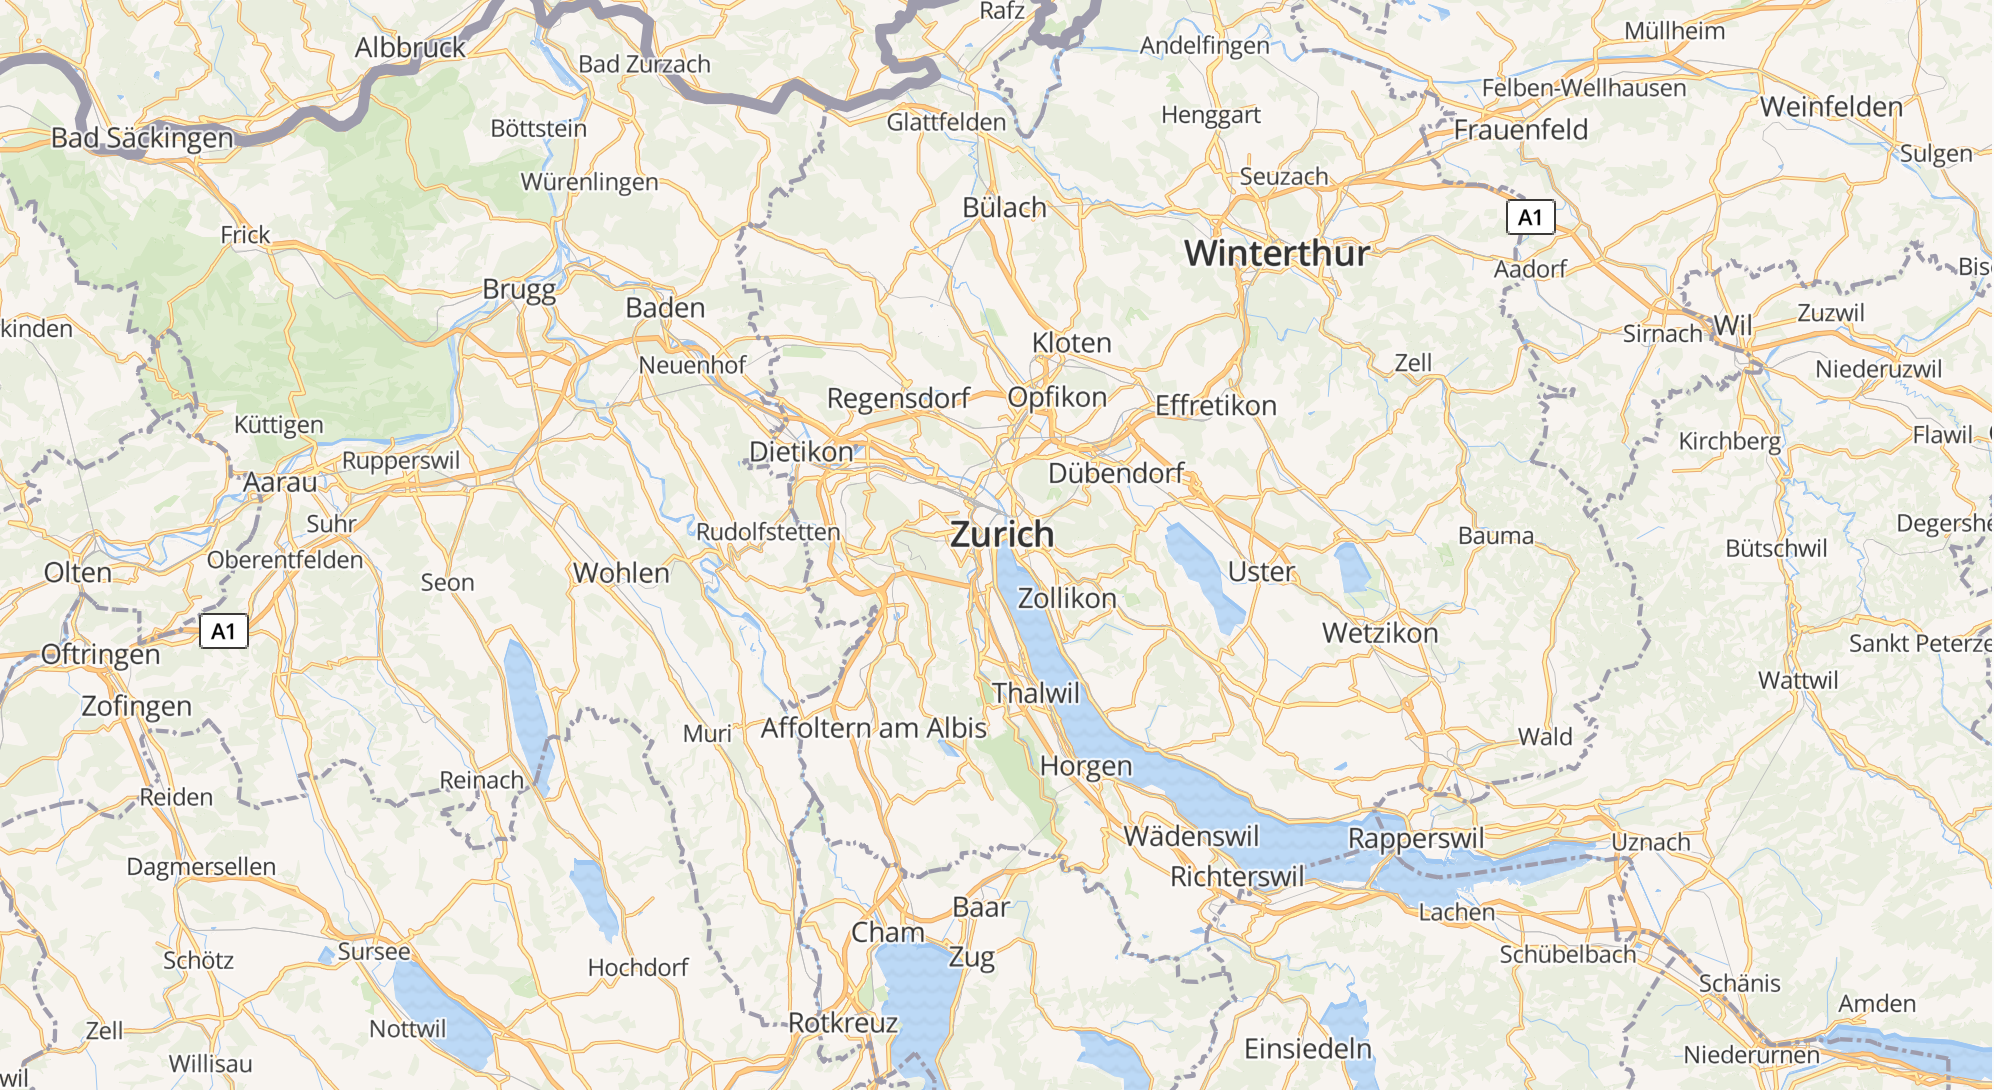
\includegraphics[width=\textwidth]{images/osm_bright}
\caption*{Map rendered from \osmvt{} vector tiles}
\end{figure}

%---------------------------------------------------
\subsection*{Approach}

The \osmvt{} project strives to push mapping forward by providing free and high quality vector tiles with no strings attached. To make developers independent from the providers
the vector tiles can be downloaded and hosted using a tileserver of their choice. This approach differs from all other vector tile providers and will enable new possibilities for desktop and mobile developers creating offline map applications.\\

The process to improve \osmvt{} is completely open and the feedback and requirements of the
community have been the cornerstone for improving the project with most feature requests and
bug reports coming from actual users.

%---------------------------------------------------
\subsection*{Result}

The result of this thesis are downloadable vector tiles for the entire world and extracts for over 200 countries and 600 cities provided on the project website \url{http://osm2vectortiles.org}. The vector tiles are compatible with the newest Mapbox Streets v7 vector tiles which allows people to use their visual styles created with Mapbox Studio together with OSM2VectorTiles.\\

The workflow to create the vector tiles is available for everyone to use and is meant to be adapted by other projects. The workflow can be scaled linearly by adding more worker machines and is a unique approach to rendering offline vector tiles with global coverage.\\

The vector tiles can be kept up to data by continuously applying the latest \osm{} changes and rerendering only the parts of the planet that are affected by those changes. This enables to provide downloadable vector tiles but still keep the data up to date.\\

The \osmvt{} project is already used in several real world projects and by pushing the project further the result of this thesis is a living open source project that hopefully will survive this bachelor thesis.
    
\begin{figure}[H]
\centering
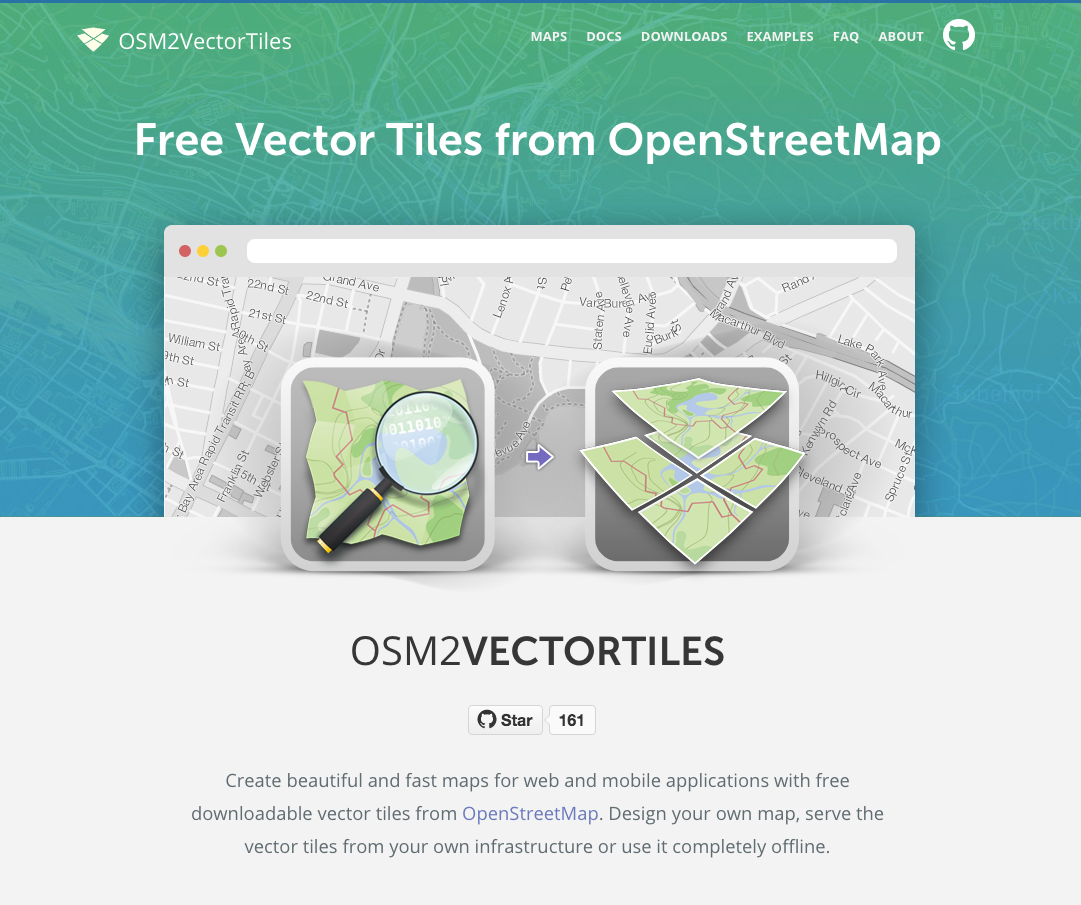
\includegraphics[width=\textwidth]{images/project_website}
\caption*{Project website \osmvt{} providing docs, downloads and examples}
\end{figure}

\endgroup

\vfill

% Acknowledgements

\pdfbookmark[1]{Acknowledgements}{Acknowledgements} % Bookmark name visible in a PDF viewer

\bigskip

%-------------------------------------------------

\begingroup

\let\clearpage\relax
\let\cleardoublepage\relax
\let\cleardoublepage\relax

\chapter*{Acknowledgements} % Acknowledgements section text

We want to thank the following people for their support and contributions to the thesis.\\

\textbf{Prof Stefan Keller, IFS Institute for Software}, for his support with regular meetings, contacts in the OSM community and time and effort in checking this thesis.\\

\textbf{Imre Samu, \osm{}}, for the help in maintaining the project, advice on technical
challenges and code contributions.\\

\textbf{Brett Davidson, PhD, HSR}, for helping us with the writing in this thesis.\\

\textbf{Petr Pridal, PhD, Klokan Technologies GmbH}, for initiating the project and donating the necessary cloud and CDN infrastructure for producing and hosting the vector tiles\\

\begin{figure}[H]
  \centering
  
\includegraphics[scale=0.3]{images/klokantech_logo.png}
  \caption*{\url{http://www.klokantech.com/}}
\end{figure}
\endgroup





\pagestyle{scrheadings} % Show chapter titles as headings

% Table of Contents - List of Tables/Figures/Listings and Acronyms

\refstepcounter{dummy}

\pdfbookmark[1]{\contentsname}{tableofcontents} % Bookmark name visible in a PDF viewer

\setcounter{tocdepth}{2} % Depth of sections to include in the table of contents - currently up to subsections

\setcounter{secnumdepth}{3} % Depth of sections to number in the text itself - currently up to subsubsections

\manualmark
\markboth{\spacedlowsmallcaps{\contentsname}}{\spacedlowsmallcaps{\contentsname}}
\tableofcontents 
\automark[section]{chapter}
\renewcommand{\chaptermark}[1]{\markboth{\spacedlowsmallcaps{#1}}{\spacedlowsmallcaps{#1}}}
\renewcommand{\sectionmark}[1]{\markright{\thesection\enspace\spacedlowsmallcaps{#1}}}

\clearpage

\begingroup 
\let\clearpage\relax
\let\cleardoublepage\relax
\let\cleardoublepage\relax

%----------------------------------------------------------------------------------------
%	List of Figures
%----------------------------------------------------------------------------------------

\refstepcounter{dummy}

%\pdfbookmark[1]{\listfigurename}{lof} % Bookmark name visible in a PDF viewer

\listoffigures

\vspace*{8ex}
\newpage

%----------------------------------------------------------------------------------------
%	List of Tables
%----------------------------------------------------------------------------------------

\refstepcounter{dummy}
\listoftables

\vspace*{8ex}
\newpage
    
%-------------------------------------
%	List of Listings
%-------------------------------------


%\refstepcounter{dummy}
\renewcommand\listoflistingscaption{List of source codes}
\listoflistings
\vspace*{8ex}
\newpage

%\addcontentsline{toc}{chapter}{\lstlistlistingname} % Uncomment if you would like the list of listings to appear in the table of contents

%\pdfbookmark[1]{\lstlistlistingname}{lol} % Bookmark name visible in a PDF viewer
%
%\lstlistoflistings 
%
%\vspace*{8ex}
%\newpage
       
%----------------------------------------------------------------------------------------
%	Acronyms
%----------------------------------------------------------------------------------------
\refstepcounter{dummy}
\markboth{\spacedlowsmallcaps{Acronyms}}{\spacedlowsmallcaps{Acronyms}}
\chapter*{Acronyms}

\begin{acronym}[Acronyms]
\acro{OSM}{OpenStreetMap, free map}
\acro{ETL}{Extract, Transform and Load}
\acro{RUP}{Rational Unified Process}
\acro{GIS}{Geographic Information System}
\acro{GDAL}{Geospatial Data Abstraction Library}
\acro{WMS}{Web Map Service}
\acro{DRY}{Don't Repeat Yourself}
\acro{CI}{Continuous Integration}
\acro{CDN}{Content Delivery Network}


\end{acronym}  

\newpage

%----------------------------------------------------------------------------------------
%	Glossary
%----------------------------------------------------------------------------------------
\refstepcounter{dummy}
\markboth{\spacedlowsmallcaps{Glossary}}{\spacedlowsmallcaps{Glossary}}
\chapter*{Glossary}

\begin{acronym}[Glossary]
\acro{Vector Tiles}{Packets of geographic data, packaged into pre-defined roughly-square shaped "tiles" for transfer over the web}
\acro{Mapbox Streets}{Name of Mapbox's vector tile source}
\acro{MBTiles}{File format for storing map tiles in a single file}
\acro{GeoJSON}{File format for encoding a variety of geographic data structures}
\acro{Mapbox GL}{Clientside rendering engine}
\acro{Web GL}{Javascript API for the graphics library in browsers}
\acro{Docker}{Operation system level virtualization on Linux}
\acro{Natural Earth}{Public map dataset}
\acro{OSM Planet}{All OpenStreetMap data in one file}






\end{acronym}  

\endgroup % Contents, list of figures/tables/listings and acronyms

\pagenumbering{arabic} % Arabic page numbering for thesis content (1, 2, 3, etc)

%------------------------------------------------
%	THESIS CONTENT - CHAPTERS
%------------------------------------------------
\newpage
\part{Technical Report}\label{technical_report}
\chapter{Introduction}

%---------------------------------------


%---------------------------------------

\section{Vision}\label{part1_vision}

Vector tiles are the future of web and mobile mapping. The next generation of maps is only possible
with free and open vector tile sources. The goal of the bachelor thesis is to push mapping forward by providing
vector tiles that are produced using an open process, completely free of charge and can be used offline.
Encouraged by the existing real users of the project further improvements need to be done to meet the requirements of developers and cartographers using the project to create custom OSM maps without building up their own rendering pipeline. These actions will lead to further adoption and a healthy Open Source project that will survive this thesis.

%---------------------------------------

\section{Problems}\label{goals}

The focus off this bachelor thesis lies on three major problems that need to be solved.


\subsection{Scalable rendering process}\label{scalable-rendering-process}

The global vector tiles should be rendered within a reasonable time-frame
to meet project deadlines and enable developers to iterate quickly on the vector tiles.
Unfortunately to the sheer amount of tiles a single process on a single machine takes a half year to complete.
By distributing the process on multiple machines the time for rendering the planet can be significantly reduced only limited
by the amount of infrastructure available serving as example how to distribute a tile rendering pipeline and enabling
vector tiles with global coverage.

\subsection{Updatable vector tiles}

\osm{} contributors add several million changesets every day. Keeping a map up to date is of significant relevance to the users of the vector tiles and the contributors. The vector tiles should be released in a fixed weekly interval.
However rerendering the entire planet using the scalable rendering process is not feasible due to the infrastructure costs. By calculating the tiles that will change in advance and only render those tiles a single machine can keep the vector tiles up to date making the project sustainable for long term. 


\subsection{Cartographic Standards}

The vector tiles need to meet certain cartographic standards to enable cartographers to create high quality maps. Creating a global base map from scratch is a huge undertaking with several interesting problems like label placement, importance ranking and fitting the right data into less space. By focusing on quality and compatibility with Mapbox Streets v7 the vector tile data schema and makes the project truly usable for the end users which expect high quality maps.
\chapter{Theory}

This chapter describes the underlying concepts which are used throughout the thesis. 

\section{Vector Tiles}\label{part1_vector_tiles}

Instead of delivering a image of the map to a client like a browser or mobile phone, only the vector representation of the data is sent to the client which is using less data and allows more interactive, dynamic  and resolution independent cartography. This is only possible since clients have more powerful hardware and are able to render maps themselves.

\begin{figure}[H]
\centering
\includegraphics[width=1.0\textwidth]{images/vector_raster_example}
\caption{Vector and client representation of a map section}
\end{figure}

Google introduced the XYZ tiling scheme \cite{v_1_wiki.openstreetmap.org_2015} back in 2005 because it is not scalable to deliver an image of the map tailored to the viewport of the client.
The idea is to divide the map image into a grid where clients request idempotent raster images by using tile indizes instead of coordinates. This allows caching on the browser and server side and results in a smoother map experience.
The same approach can be applied to vector data. Instead of delivering the vector data for the entire viewport the vector data is sliced into tiles. \\\\

\begin{figure}[H]
\centering
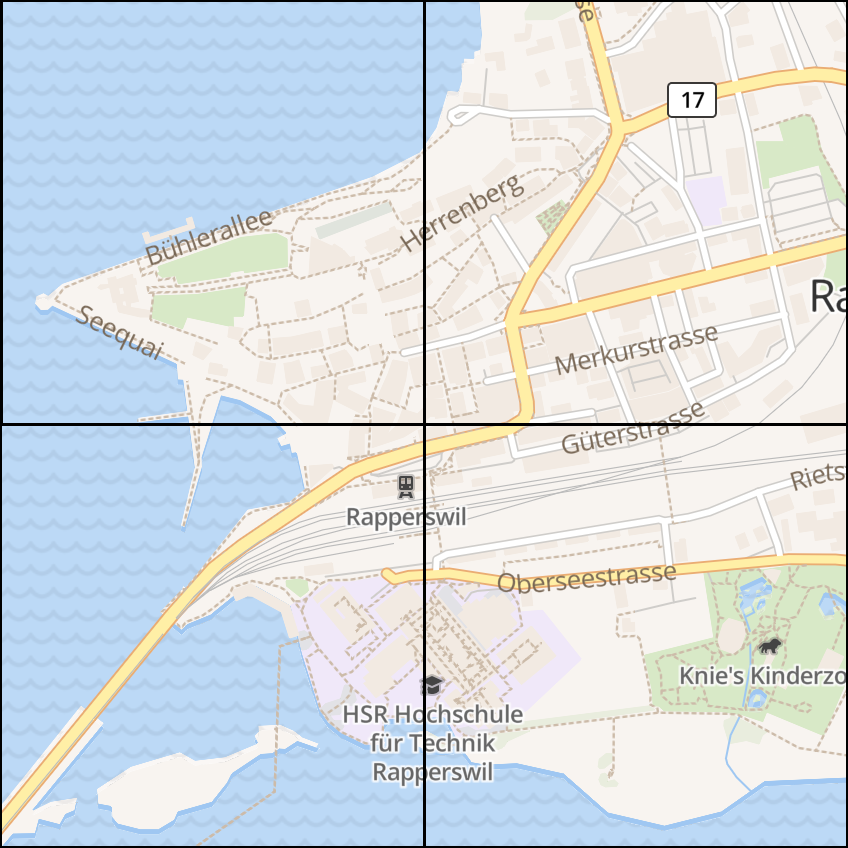
\includegraphics[width=0.5\textwidth]{images/tiled_raster}
\caption{Tiled raster map}
\end{figure}

Vector tiles contain all the geometry and metadata needed for a specific tile. This makes them more flexible than serving raster tiles, because a different style can be applied on the fly. For example based on the language preference of the browser language-specific city labels can be shown.\\

The data inside of vector tiles is structured into layers and features. A vector tile can have multiple layers such as roads, landuse or water (elaborated in \autoref{database-schema}). Each layer consist of one or multiple features. A feature contains a geometry field (either of type point, linestring or polygon) and metadata such as label translations.

\subsection*{Mapbox Vector Tile Specification}\label{part1_vector_tile_specification}

The Mapbox Vector Tile Specification defines how to encode tiled vector data using Protobuf. More details about the encoding and internal structure of vector tiles can be found in the specification\cite{104_mapbox.com_2016}.

\section{XYZ Coordinate Schema}\label{part1_xyz_coordinates}

For tiling the vector tiles the XYZ numbering schema has been used.
The tiles are organized in a 3-dimensional coordinate system (\texttt{x/y/z}) where \texttt{x} and \texttt{y} represent the axes and \texttt{z} the zoom level. As users zoom into a map each tile is replaced by four children within the tile.

\begin{figure}[H]
\centering
\includegraphics[width=0.5\textwidth]{images/xyz_scheme}
\caption{XYZ coordinate schema}
\end{figure}

\section{OpenStreetMap Data Model}\label{openstreetmap_data_model}

The data model of \osm{} consists of objects of type node, way and relation. Nodes define points in space, ways define linear features and relations define how objects relate to each other\cite{1_osm_wiki_2016}.

\begin{figure}[H]
\centering
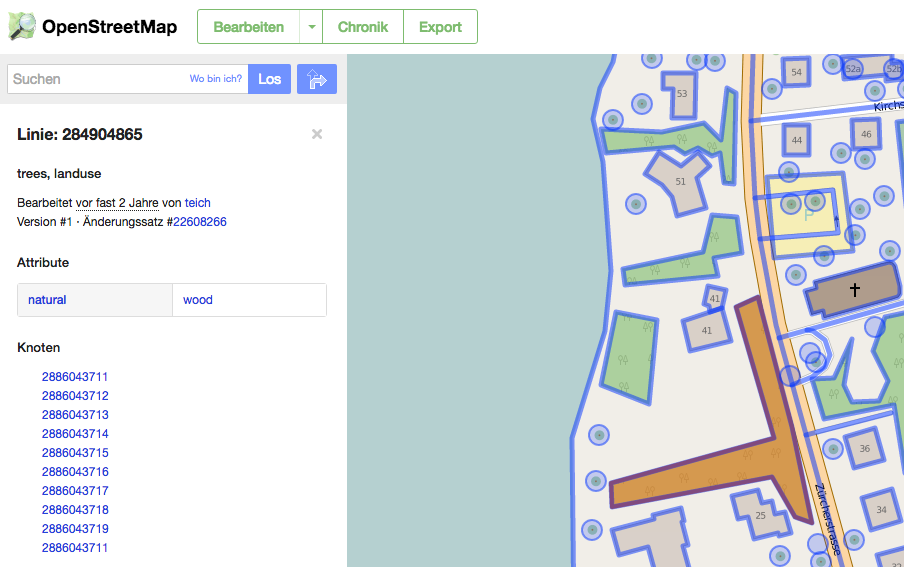
\includegraphics[width=0.8\textwidth]{images/osm_data_model}
\caption{Example of object tagged with natural=wood}
\end{figure}

Every object can have one or more tags associated with it. Tags define the meaning of a certain object. A tag consists of a key/value pair for example the tag \textbf{natural=wood} is used to define areas which are covered in trees. OSM tags are not strictly defined and users can add their own tags but there are many conventions which should be followed.
\chapter{Defining Mapbox Vector Tiles}\label{chapter_defining_mapbox_vector_tiles}

The main requirement regarding the content of the vector tiles is to be compatible with the vector tiles of Mapbox. This allows people to seamlessly switch to \osmvt{} and use the same visual styles created with Mapbox Studio. 

\section{Approach}
Mapbox's tileset is called Mapbox Streets. They provide detailed documentation on what data is included in the Mapbox Streets vector tiles. The documentation contains a layer reference which defines the attributes a layer can have. However the zoom levels at which data is shown is not documented publicly as well as the \osm{} tags and constraints describing the data. To be able to reverse engineer Mapbox Streets this information had to be retrieved by analyzing the official Mapbox Streets vector tiles at different zoom levels.\\
In an iterative and time consuming process the mapping and queries were continuously improved until the vector tile output matches the data from Mapbox Streets very closely.

\section{Implementation}
This section describes the main components which needed to be implemented in order to generate Mapbox Streets compatible vector tiles.

\begin{figure}[H]
\centering
\includegraphics[width=1.0\textwidth]{images/osm_to_vectortiles_detailed}
\caption{Simplified process of data import to vector tile rendering}
\end{figure}

\clearpage

\subsection{Import Mapping}

Imposm3 is used to import the \osm{} data into the Postgres database. Imposm3 expects a definition of which \osm{} tags should be mapped to which database tables. This definition is called import mapping. It mainly satisfies the following two purposes:

\paragraph{Filter data} The mapping allows to declare which data needs to be imported. This is very important since only a subset of all \osm{} data is included in the vector tiles. Therefore not all \osm{} data needs to be imported.

\paragraph{Mapping data} The mapping allows to map \osm{} key/value pairs to a certain database table creating a structured and organized schema from unstructured data.\\

The example definition in listing \autoref{definition_of_mapping} maps \osm{} tags with the key \textbf{aeroway} and one of the values \textbf{runway}, \textbf{taxiway}, \textbf{apron} or \textbf{helipad} to the table \textbf{aero\_polygon}. The \textbf{aero\_polygon} table has the columns \textbf{id}, \textbf{geometry}, \textbf{timestamp} and \textbf{type}. During the import process Imposm3 transformes the \osm{} nodes, ways and relations to one of the geometry types point, linestring or polygon.

\begin{listing}[H]
\begin{yamlcode}
aero_polygon:
  type: polygon
  fields:
  - name: id
    type: id
  - name: geometry
    type: geometry
  - name: timestamp
    type: pbf_timestamp
  - name: type
    type: mapping_value
  mapping:
    aeroway:
    - runway
    - taxiway
    - apron
    - helipad
\end{yamlcode}
\caption{Definition of a single table in the import mapping}
\label{definition_of_mapping}
\end{listing}
\clearpage

\subsection{Zoom Level Views}

Since only a subset of the data in the tables is shown on a given zoom level, SQL views for each zoom level were created. The figure \ref{definition_of_zoom_level_view} shows the definition of the SQL view for zoom level 9 of the aeroway layer. The zoom level view merges the data of both tables osm\_aero\_linestring and osm\_aero\_polygon and filters the data to only contain geometries of type runway.

\begin{listing}[H]
\begin{sqlcode}
CREATE OR REPLACE VIEW aeroway_z9 AS
    SELECT id AS osm_id, type, geometry
    FROM osm_aero_linestring
    WHERE type = 'runway'
    UNION ALL
    SELECT id AS osm_id, type, geometry
    FROM osm_aero_polygon
    WHERE type = 'runway';
\end{sqlcode}
\caption{Definition of zoom level view}
\label{definition_of_zoom_level_view}
\end{listing}

The zoom level views help to decouple the database tables which hold the actual data and the definition of the layer. This is very helpful for example if new data is added to a layer, as only the import mapping and the zoom level view needs to be modified.

\subsection{Layer Definition}

The source project contains the definition of the layers inside the vector tiles. The definition contains metadata to access the database and a query which returns the necessary data for this layer. The listing \autoref{definition_of_layer} shows the definition of the layer \textbf{aeroway}. The query does not directly access the database table \textbf{aero\_polygon} instead it queries the zoom level views \textbf{aeroway\_z9} and \textbf{aeroway\_z10to14}.

\begin{listing}[H]
\begin{yamlcode}
- id: aeroway
    Datasource: 
      dbname: osm
      host: db
      password: osm
      port: 5432
      table: |-
        (
          SELECT osm_ids2mbid(osm_id, is_polygon(geometry)) AS osm_id, geometry, type
          FROM (
            SELECT * FROM aeroway_z9
            WHERE z(!scale_denominator!) = 9
            UNION ALL
            SELECT * FROM aeroway_z10to14
            WHERE z(!scale_denominator!) BETWEEN 10 AND 14
          ) AS aeroway WHERE geometry && !bbox!
        ) AS data
      type: postgis
      user: osm
    properties: 
      "buffer-size": 4
\end{yamlcode}
\caption{Definition of layer aeroway}
\label{definition_of_layer}
\end{listing}

This layer definition serves as input to the vector tile renderer (Mapnik). The tile renderer will execute every layer query for each tile and replaces expressions like \textbf{!scale\_denominator!} (zoom level) and \textbf{!bbox!} (extent of the tile) with the values of the current tile. If the query above gets executed for a tile on zoom level 8 it won't return any data as the \textbf{WHERE} clause will return in both case false. Whereas if it gets executed on a tile on zoom level 9 all data of the zoom level view aeroway\_z9 will be included in the layer aeroway.

\subsection{Conclusion}

The \autoref{aero_db_schema} below shows how the database tables, zoom level views and layers are related to each other. This architecture helps to structure the \osm{} data inside the database and opens the possibility to optimize single zoom levels individually.

\begin{figure}[H]
\centering
\includegraphics[width=0.8\textwidth]{images/aero_database_schema}
\caption{Relations between database tables, zoom level views and layer}
\label{aero_db_schema}
\end{figure}

\section{Problems and Optimizations}

During the development process of the map a number of problems were discovered and optimizations were implemented. This section explains the most interesting problems in detail.

\subsection{Avoid expensive Functions in Zoom Level Views}

The purpose of the zoom level views is to filter the data to only contain rows that are shown on a specific zoom level. Expensive calculations or transformations should be avoided in these views.\\
For example there are multiple label layers which transform a polygon geometry to a point geometry. Doing transformations like these in the zoom level views results in bad rendering performance. 
The reason for this is that every time the layer query gets executed all rows of the view are transformed and only then most of the rows were discarded because they didn't fit in the bounding box. So first selecting the right row and only executing the transformation on this subset resulted obviously in way better performance.

\begin{figure}[H]
\centering
\includegraphics[width=1.0\textwidth]{images/expensive_functions}
\caption{Example of expensive function which was moved into the layer query}
\end{figure}

\begin{tcolorbox}[arc=0mm,boxrule=1pt,title=Learning]
Expensive transformations should either be  made in a preprocessing step or if that's not possible the dataset should be reduced to the smallest size possible.
\end{tcolorbox}
\clearpage

\subsection{Helper functions}

Small helper functions were created to make the queries more readable and secondly to reuse common logic through multiple queries.\\ 
Mapbox has introduced a complex classification schema to be able to filter features of a single layer. For example the layer landuse contains features of class park, school, cemetery and many more. This allows people to style these areas differently. OpenStreetMap has an entirely different data model. Therefore a helper function was created to assign the right class value to each row.

\begin{listing}[H]
\begin{sqlcode}
CREATE OR REPLACE FUNCTION landuse_class(type VARCHAR) RETURNS VARCHAR
AS $$
BEGIN
    RETURN CASE
        WHEN type IN ('park', 'dog_park', 'garden', 'playground') THEN 'park'
        WHEN type IN ('school', 'college', 'university') THEN 'school'
        WHEN type IN ('cemetery', 'christian', 'jewish') THEN 'cemetery'
    END;
END;
$$ LANGUAGE plpgsql IMMUTABLE;
\end{sqlcode}
\caption{Definition of classification helper function}
\label{definition_of_classification_helper_function}
\end{listing}

The listing \autoref{definition_of_classification_helper_function} shows the simplified class function of the layer landuse it takes the type value as input and returns the correct class value. 

\paragraph{Expensive helper functions} In many cases these helper functions are used inside the zoom level views. For example from zoom level 5 to 6 only rows of class wood are shown. It turned out that this function introduced a bottleneck. The function could not be moved to the layer query like the example with the ST\_PointOnSurface transformation above, because it is used to filter the data. So an index on the stored procedure was created which improved the performance.

\begin{listing}[H]
\begin{sqlcode}
CREATE OR REPLACE VIEW landuse_z5toz6 AS
    SELECT id AS osm_id, geometry, type
    FROM osm_landuse_polygon_gen0
    WHERE landuse_class(type) = 'wood';
\end{sqlcode}
\caption{Definition of landuse zoom level view}
\label{definition_of_landuse_zoom_level_view}
\end{listing}
\clearpage

\subsection{OpenStreetMap ID Transformation}

The data model of \osm{} consists of nodes, ways and relations. Every object gets its own OSM ID assigned. This OSM ID is not unique across object types. Therefore one can find three objects with the same OSM ID but with a different object type.\\
While this works perfectly fine for \osm{}, this represents a problem because during the import process as the \osm{} objects get transformed to PostGIS geometries. For example an object of type way and relation could get transformed to a linestring geometry.

In order to ensure that the \osm{} ID remains the IDs need to be transformed according to \autoref{osm_id_transformation} into the same ID space Mapbox is using to make OSM IDs unique within vector tiles \cite{103_mapbox.com_2016}.

\begin{table}[H]
\centering

\begin{tabular}{lll}
\hline
OSM type & Geometry type                  & \osm{} ID transform \\ \hline
node     & point                          & id x 10          \\
way      & linestring                           & (id x 10) + 1    \\
way      & polygon + polygon label points & (id x 10) + 2    \\
relation & linestring                           & (id x 10) + 3    \\
relation & polygon + polygon label points & (id x 10) + 4    \\
\end{tabular}
\caption{OSM id transformation}
\label{osm_id_transformation}
\end{table}

\subsubsection*{Algorithm}
Input: OpenStreetMap osm\_id\\
Output: Mapbox osm\_id
\begin{enumerate}
    \item If osm\_id is point geometry return osm\_id * 10
    \item If osm\_id has object type way and was transformed to linestring\\
    return (osm\_id * 10) + 1
    \item If osm\_id has object type way and was transformed to polygon\\
    return (osm\_id * 10) + 2
    \item If  osm\_id has object type relation and was transformed to linestring\\
    return (osm\_id * 10) + 3
    \item If osm\_id has object type relation and was transformed to polygon\\
    return (osm\_id * 10) + 4
\end{enumerate}

\clearpage
\subsection{Place Label Rank Calculation}

Ranks are important for determining at which zoom level which places should be displayed. The NaturalEarth database contains places with scaleranks assigned by humans and is the most important source for better quality labels (historic places might be much more important despite having a very small population). This dataset is merged with the imported \osm{} data.
They can also be used to limit density at lower zoom levels to decrease data density.

\subsubsection*{Algorithm}

\begin{enumerate}  
    \item Divide map into grid
    \item Group labels by tile index
    \item Sort labels by scalerank, type and population within group
    \begin{enumerate}
        \item By scalerank ascending
        \item By type city, town, village, hamlet, suburb, neighbourhood
        \item By population descending
    \end{enumerate}
    \item Assign row number as \texttt{localrank}
\end{enumerate}


\begin{figure}[H]
\centering
\includegraphics[width=0.75\textwidth]{images/rank_calculation.png}
\caption{Local place rank calculation}
\end{figure}


\chapter{Scalable Rendering Process}

\section{Jobs}

To render the entire planet the work must be divided.
The export process at the most basic level takes a bounding box and renders just
the tiles from this section of the entire planet into the MBTiles SQLite database.
Each job therefore consists of either a bounding box derived from a tile (pyramid job) or a list of tiles (list job).

\begin{figure}[H]
  \centering
  \includegraphics[width=0.7\textwidth]{images/bbox_to_tile.png}
  \caption{Mapnik renders bounding box from planet into SQLite database}
\end{figure}

\begin{figure}[H]
  \centering
  \includegraphics[width=0.84\textwidth]{images/distributed_export_process.png}
  \caption{Distributed rendering process using message queues}
\end{figure}

\section{Merging Results}

Each job is producing a SQLite database container with the tiles stored.
To merge the different databases together into one large database the SQLite \texttt{REPLACE INTO} is used.

\begin{figure}[H]
  \centering
  \includegraphics[width=0.88\textwidth]{images/merge-jobs.png}
  \caption{Merge completed MBTiles files together}
\end{figure}


\subsection{Pyramid Job}

To divide the work for rendering the planet into equal parts across the world we use the XYZ tiling scheme and divide the planet into several subpyramids.

\subsubscection{Algorithm}

\begin{enumerate}  
    \item Choose job zoom level
    \item Calculate all the tiles for job zoom level
    \item Render subpyramid from job zoom level down to max zoom level
\end{enumerate}

\begin{figure}[H]
  \centering
  \includegraphics[width=0.8\textwidth]{images/pyramid_job.png}
  \caption{Pyramid job of a zoom level 2 tile and the descendants}
\end{figure}

\subsubscection{Example}

Given the job zoom level z8 and the max zoom level z14 the planet is divided into $4^{8}$ jobs.
This means each subpyramid tasks consists of rendering all descendant tiles from a z8 tile.
Each task therefore consists of 5461 tiles ($4^{0}+4^{1}+4^{2}+4^{3}+4^{4}+4^{5}+4^{6}$). \\

\begin{figure}[H]
  \centering
  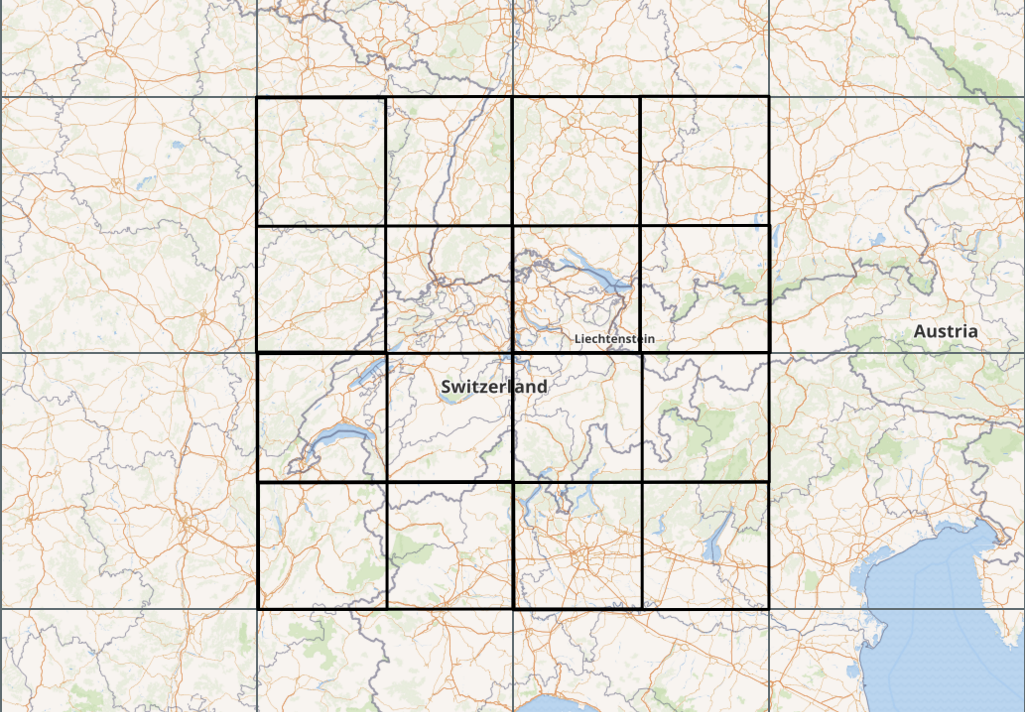
\includegraphics[width=0.8\textwidth]{images/switzerland_tiled_z8.png}
  \caption{Map divided into z8 tiles}
\end{figure}

\section{List Job}

\chapter{Updatable Vector Tiles}\label{chapter_updatable_vector_tiles}


\osm{} contributors add more than three million nodes and ways every day.
In order to keep the prerendered tiles up to date this poses a challenge of looking at the changes
and figuring out which tiles are affected by those changes and schedule them for rerendering.

\begin{figure}[H]
  \centering
  \includegraphics[width=1.0\textwidth]{images/updatable_vectortiles_flow.png}
  \caption{Simplified diagram of changed tiles detection process}
\end{figure}

To find out which tiles are affected by updates requires a multi-step process.

\begin{enumerate}
    \item Find relevant \osm{} objects affected by the changes
    \item Calculate tiles covered by the object geometries
\end{enumerate}

\paragraph{Time Constraint} In order to be able to keep up with rendering changes the update process can not take longer than the number of days the database is behind.

\section{OSM Diff File}

\osm{} provides a single XML file, which contains every mapped object. Since the process of importing is time and resource consuming it is not feasible to redo this process to keep up with all the changes. Therefore OSM additionally provides hourly or daily diff files in the OsmChange format which contains the created, modified and deleted objects over a period of time. Importing only the subsequent diff files after an initial import allows to keep the database in sync with the latest changes.

\subsection*{Example}
The listing \autoref{create_modify_delete_xml} shows an example diff file which contains a create, modify and delete entry for different objects.

\begin{listing}[H]
  \centering
  \begin{xmlcode}
<?xml version='1.0' encoding='UTF-8'?>
<osmChange version="0.6" generator="Osmosis 0.43.1" timestamp="2016-05-20T11:32:32Z">
  <create>
    <node id="4196907493" version="1" uid="1" lat="46.9280366" lon="7.1163806">
      <tag k="amenity" v="pharmacy"/>
      <tag k="name" v="Amavita"/>
    </node>
  </create>
  <modify>
    <node id="4051684660" version="2" uid="1" lat="53.5705074" lon="9.9950888">
      <tag k="emergency" v="fire_hydrant"/>
      <tag k="ref" v="13874"/>
    </node>
    </modify>
  <delete>
    <node id="1044604768" version="2" uid="1" lat="52.6429848" lon="5.082264"/>
  </delete>
</osmChange>
  \end{xmlcode}
  \caption{Create, modify and delete example}
  \label{create_modify_delete_xml}
\end{listing}

\subsection*{Different Change scenarios}\label{osm_change_scenarios}


\paragraph{Create object} A new object is created (e.g. a new point of interest is added). All tiles covered by the created object must be rerendered.

\paragraph{Delete object} An object gets deleted (e.g. an old house which does not exist anymore). All tiles covered by the deleted object must be rerendered.

\paragraph{Modify object} An object gets modified (e.g. add additional translations to a place). All tiles covered by the modified object must be rerendered.

\paragraph{Move object} An object is moved (e.g. an incorrectly mapped bus stop had to be repaired or has been moved in the real world). All tiles covered by the original object and all tiles covered by the moved object must be rerendered.

\section{Diff Import}

Imposm3 is used for the regular import of the OSM Planet file. Additionally it supports importing OSM Diff files. Imposm3 will read the XML File and calculate with the local cache of previous imports which nodes, ways and relations are affected by the changes.

If the changes would be mapped into the database existing entries in the database will first be removed using a SQL \texttt{DELETE} and then added again using SQL \texttt{INSERT}.\\\\

\begin{figure}[H]
  \centering
  \includegraphics[width=0.35\textwidth]{images/imposm3_operations_venn_diagram.png}
  \caption{Imposm3 SQL statements and OSMChange actions}
\end{figure}

The diff import functionality of imposm3 is only meant to keep the database in sync with the OSM changes. It is not possible to track which rows in the table have been inserted, updated or deleted. However this information is crucial to detect changed tiles and support all change scenarios from \autoref{osm_change_scenarios}.
The only way to keep track of changed features is to either modify Imposm3 or take actions at the database level.

\subsection{Track changes}

To track the entries at the database level the timestamp of the import is added to each object. This makes it possible to query modified and created objects by filtering for the latest import date.

To keep track of entries that are no longer present in the database (like deleted and moved objects) auditing of \texttt{DELETE} actions has been implemented.

\subsubsection{Track inserted rows}

The \texttt{timestamp} column is used to keep a history of inserted features. The \texttt{timestamp} column contains the date of the original PBF or OSC file the feature was defined or changed. This is important for calculating the changed tiles in a timeframe later on in \autoref{calculate-changed-tiles}.

\begin{enumerate}
   \item The imposm3 diff process inserts new rows for updated and added features
   \item The \texttt{timestamp} column is now set to \texttt{NULL} for all new rows
   \item Update the table and set the rows \texttt{timestamp} column to the timestamp of the import
\end{enumerate}

\subsubsection{Track deleted rows}

If \osm{} features are changed or removed imposm3 will first delete the row from the table and then insert it again (if it is an update). This is due to performance reasons since a \texttt{DELETE} followed by an \texttt{INSERT} is faster than an \texttt{UPDATE}.

To support the change scenarios of deleting, modifying and moving an object the \texttt{track\_osm\_delete} trigger is enabled for each table to keep track of deleted rows (similar to database auditing).

\begin{listing}[H]
  \centering
  \begin{sqlcode}
    DROP TRIGGER IF EXISTS osm_building_polygon_track_delete ON osm_building_polygon;
    CREATE TRIGGER osm_building_polygon_track_delete
    BEFORE DELETE ON osm_building_polygon
    FOR EACH ROW EXECUTE PROCEDURE track_osm_building_polygon_delete()
  \end{sqlcode}
  \caption{Delete trigger on a table}
\end{listing}

The trigger will track the deleted row in a separate audit table before discarding it.

\begin{listing}[H]
  \centering
  \begin{sqlcode}
CREATE OR REPLACE FUNCTION track_osm_building_polygon_delete() RETURNS TRIGGER AS $$
BEGIN
     IF (TG_OP = 'DELETE') THEN
        INSERT INTO osm_building_polygon_delete(id, geometry)
        VALUES($1, $2) USING OLD.id, OLD.geometry;
        RETURN OLD;
     END IF;
     RETURN NULL;
END;
$$ language plpgsql;

  \end{sqlcode}
  \caption{Logic of delete trigger}
\end{listing}

As a result each table has an additional delete tables which contains all deleted and modified rows. This allows in a second step to calculate the affected tiles and rerender them.

%----------------------------
\newpage{}
\section{Calculate changed tiles}\label{calculate-changed-tiles}

One way to determine which tiles are affected by changes in the database is to calculate the covered tiles from changed geometries by recursively descending the XYZ Quadtree and checking for intersections of the tiles and geometries.

\subsubsection*{Algorithm}

\begin{enumerate}  
    \item \label{itm:calc-extent}Calculate the extent $e$ for a given $(x,y,z)$ tile index
    \item \label{itm:bbox} Check if geometry $g$ intersects with the tile extent $e$ 
    \item Stop if there is no intersection in \ref{itm:bbox}
    \item Select tile index $(x,y,z)$
    \item Calculate the four child XYZ indizes \\
       \begin{pmatrix}
            x*2 & y*2 & z+1\\
            x*2+1 & y*2 & z+1\\
            x*2 & y*2+1 & z+1 \\ x*2+1 & y*2+1 & z+1
        \end{pmatrix}
    \item Call \ref{itm:calc-extent} for children if zoom level $z$ has not reached max zoom level $Z$
\end{enumerate}

\begin{figure}[H]
  \centering
  \includegraphics[width=0.9\textwidth]{images/polygon_xyz_matching.png}
  \caption{Recursive tile matching on polygon}
\end{figure}

\subsubsection*{Tile Buffers}

Geometries in vector tiles can extend beyond the boundaries of a tile (tile buffer).
To support the concept of a buffer in the algorithm the extent $e$ for the $(x,y,z)$ tile index
is extended by a custom buffer $b$. The tile usually has a resolution of $256$px. By adding the buffer to the tile $256 + 2 * b$ it is ensured that tiles that contain the geometries inside their buffers are detected as well.

\begin{figure}[H]
  \centering
  \includegraphics[width=0.7\textwidth]{images/polygon_buffer_xyz_matching.png}
  \caption{Recursive buffered tile matching on polygon}
\end{figure}


\subsubsection*{PostgreSQL Implementation}

The PostGIS implementation makes heavy use of the \texttt{\&\&} operator and GiST indizes on the geometry columns to check whether the tile extent and geometry intersect with each other. Although using the bounding box of the geometry is not accurate and can yield false positive changed tiles it is much faster than using the correct \texttt{ST\_Intersects}.

\begin{listing}[H]
  \centering
  \begin{sqlcode}
CREATE OR REPLACE FUNCTION overlapping_tiles(geom geometry, max_zoom_level INT, buffer_size INT)
RETURNS TABLE (tile_z INT, tile_x INT, tile_y INT) AS $$
BEGIN
    RETURN QUERY
        WITH RECURSIVE tiles(x, y, z, e) AS (
            SELECT 0, 0, 0, geom && XYZ_Extent(0, 0, 0, buffer_size)
            UNION ALL
            SELECT x*2 + xx, y*2 + yy, z+1,
                   geom && XYZ_Extent(x*2 + xx, y*2 + yy, z+1, buffer_size)
            FROM tiles, (VALUES (0, 0), (0, 1), (1, 1), (1, 0)) as c(xx, yy)
            WHERE e AND z < max_zoom_level
        )
        SELECT z, x, y FROM tiles WHERE e;
END;
$$ LANGUAGE plpgsql IMMUTABLE;
  \end{sqlcode}
  \caption{Recursive tile matching of geometry}
\end{listing}


\subsection{Point Optimization}

Points always fit into a single tile at each zoom level.
Therefore given a point the covered tile can immediately be calculated. The recursive descend algorithm is not needed for this.

\begin{figure}[H]
  \centering
  \includegraphics[width=0.9\textwidth]{images/point_xyz_matching.png}
  \caption{Tiles covering a point geometry}
\end{figure}


\begin{listing}[H]
  \centering
  \begin{ccode}
#include "math.h"
float8 D2R = M_PI / 180.0;

// Latitude and longitude of Zurich
int32 zoom_level = 14;
float8 lat = 47.376887;
float8 lon = 8.541694;

float8 _sin = sin(lat * D2R);
float8 z2 = pow(2, zoom_level);

// XYZ Tile index calculated from latitude and longitude
int32 x = floor(z2 * (lon / 360 + 0.5));
int32 y = floor(z2 * (0.5 - 0.25 * log((1 + _sin) / (1 - _sin)) / M_PI));

  \end{ccode}
  \caption{Calculate tile at given zoom level for a point}
\end{listing}

\subsection{Export changed tiles}

The algorithm defined in \autoref{calculate-changed-tiles} is applied over all geometries that have changed since a given timestamp to find out all unique tiles that are affected by the changes and need to be rendered again.

\begin{listing}[H]
  \centering
  \begin{sqlcode}
    SELECT DISTINCT t.tile_x AS x, t.tile_y AS y, t.tile_z AS z
    FROM osm_building_polygon AS g
    INNER JOIN LATERAL overlapping_tiles(g.geometry, 14, 4) AS t
    ON g.timestamp >= (LOCALTIMESTAMP - INTERVAL '7 days')
  \end{sqlcode}
  \caption{Calculate all tiles containing building polygons that changed in the last 7 days}
\end{listing}

\begin{figure}[H]
  \centering
  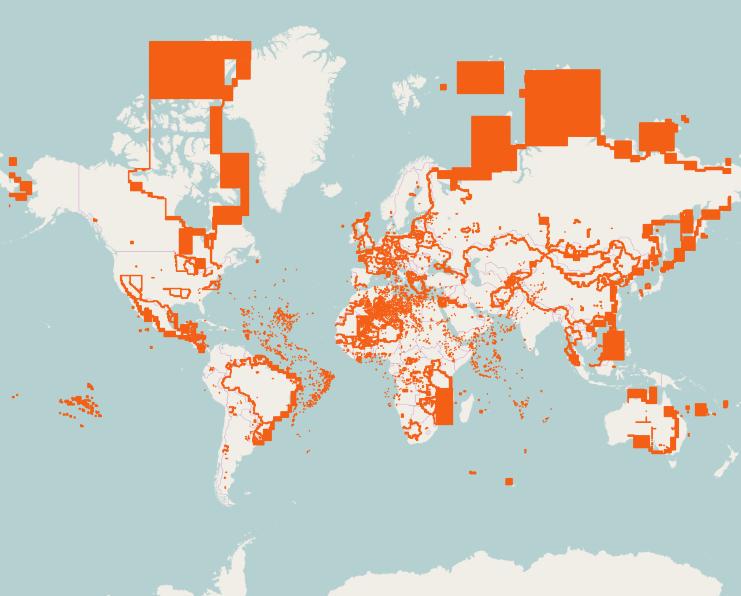
\includegraphics[width=1\textwidth]{images/changed_tiles_z10.png}
  \caption{Changed tiles on z10 over course of 10 days}
\end{figure}

\chapter{Results and Future}\label{part1_results_and_future}

All objectives which we defined in section \nameref{goals} have been achieved. The optional goal to provide vector tiles for the entire world has been moved to the bachelor thesis.

\section{Results}\label{part1_results}


\section{Future}\label{part1_future}

Future outcome is very important.
5-6 sentences. Point to a separate future chapters if necessary.


%------------------------------------------------
\newpage
\part{Project Documentation}
\chapter{Requirements Specification}\label{requirements_specification}

This chapter describes the requirements for the project.

\section{Use Cases}\label{use_cases}

There are two main use cases for this project with use case described in \autoref{use_case_use_vector_tiles} being the most relevant one while use case described in \autoref{use_case_render_vector_tiles} is for a much narrower audience.

\subsection{Render Vector Tiles}\label{use_case_render_vector_tiles}

The user renders her/his own set of vector tiles. Since not all data of \osm{} is inside our vector tiles, some users my want to remove or add additional data. Assuming users that are interested in creating their own vector tiles clone the \osmvt{} repository these are potentially ~70 users each month.

\subsection{Use Vector Tiles}\label{use_case_use_vector_tiles}

The user makes use of the prerendered vector tiles and wants to create her/his own basemap. Assuming users that are interested in using their own vector tiles read the documentation these are potentially ~600 users each month.

\section{User Characteristics}\label{user_characteristics}

\subsection{Limited or no access to the internet}

Users which have the constraint of limited or no access to the internet can download vector tiles for the entire planet and serve their custom basemap locally.

\subsection{Can't rely on a third-party service}

Many organizations can't afford to rely on a third-party service and want to run their map on-premise.

\subsection{Customizing the look of the basemap}

In many use cases it is desirably to adjust the basemap to better match the design of a product.

\section{Requirements}\label{requirements}

The bachelor thesis consists out of three major requirements out of the use cases described in \autoref{use_cases}. The technically interesting problems of these requirements are described in \autoref{technical_report}.

\begin{itemize}
    \item Prerendered vector tiles from \osm{} for the entire planet (\autoref{chapter_scalable_rendering_process})
    \item Update functionality to keep up with future \osm{} changes (\autoref{chapter_updatable_vector_tiles})
    \item Vector Tiles compatible with Mapbox Streets v7 (\autoref{chapter_defining_mapbox_vector_tiles})
\end{itemize}


\section{Non Functional Requirements}\label{non_functional_requirements}

The non functional requirements are the key to success of this project. If the following requirements can be fulfilled, the specified users will be able to benefit form our project.

\paragraph{Performance}

The initial rendering process for the entire world must be kept below two weeks. The import on the master server should take less than a day while rendering should be kept below two weeks.
Updates should happen in a weekly interval.

\paragraph{Learnability}

It is important that users without previous vector tiles or Docker experience can get started with as few obstacles as possible.

\paragraph{Cost}

The cloud instances to render the world once costs around 1500 dollar. The updating should only cost a fraction of this initial investment.

\paragraph{Repeatability}

Since the \osmvt{} will provide continuous updates it is important that the process and results are repeatable.

\paragraph{Compatibility}

Compatibility with Mapbox Streets gives the users access
to a wide range of styles and editors. Therefore the vector tiles must contain
all features sets Mapbox Streets contains.

\paragraph{Vector Tile Size}

The size of a single vector tile should not be greater than 500 KB.
\newpage
\chapter{Architecture and Design}\label{design}

\section{Architecture}

The architecture of the project is structured into the import phase (ETL process), the changed tiles detection phase  and the export phase (render vector tiles). This section describes the components and their purpose.

\begin{figure}[H]
  \centering
  \includegraphics[width=1.0\textwidth]{images/etl_components}
  \caption{Workflow structured into components}
\end{figure}

Each component is a Docker image\cite{docker} with a single purpose. The Docker containers (components) are then linked against the database container and provided with additional input data to perform their functions. Isolating the components into Docker images makes it possible to ensure that the complicated installations and dependencies of some components never cause an issue. By additionally using Docker Compose it is possible to define the entire ETL process with different containers and make deployment and scaling containers easy.

\subsection{Import Components}

The import components take care of importing \osm{} data, external data sources and SQL utilities such as views, triggers, indices and functions to help with the rendering and changed tiles detection process.

\subsubsection{Import External}

The \textbf{import-external} component is responsible for importing all data that is not mapped directly from \osm{} into the PostGIS database. \autoref{import_external_diagram} shows the external data sources and programs used to import the data into the PostGIS database. The GDAL tool ogr2ogr is used to import the various data sources into the PostGIS database.

\begin{figure}[H]
  \centering
  \includegraphics[width=1.0\textwidth]{images/architecture/import_external_diagram}
  \caption{Import of external data sources}
  \label{import_external_diagram} 
\end{figure}

\subsubsection{Import OSM}

The \textbf{import-osm} component takes the first PBF file in the import folder and imports it into PostGIS. After that it updates the scaleranks using Natural Earth data from \texttt{import-external} to update the scaleranks and create generalized tables based off the imported data. The data is imported using imposm3 diff mode and can take up to 14 hours for the entire planet file.

\begin{figure}[H]
  \centering
  \includegraphics[width=1.0\textwidth]{images/architecture/import_osm_diagram}
  \caption{Import OSM diagram}
\end{figure}

\subsubsection{Import SQL}

The \textbf{import-sql} component is responsible for provisioning the SQL used in the different layers. It also generates SQL code for different classifications and code to detect changed tiles as well as table management commands for different layers.

\begin{figure}[H]
  \centering
  \includegraphics[width=1.0\textwidth]{images/architecture/import_sql_diagram}
  \caption{Import SQL diagram}
\end{figure}

\subsection{Changed Tile Detection Components}

The changed tile detection components handle creating an \osm{} Diff file based on a certain \osm{} planet file, importing a \osm{} Diff file and updating outdated \osm{} planet file with the latest changes. The following sections show what happens in every component.

\subsubsection{Update OSM Diff}

The \textbf{update-osm-diff} component takes the planet file as input and creates an \osm{} Diff file containing all the changes happened since the planet file was downloaded. The \texttt{osmupdate} tool is used to execute this task.

\begin{figure}[H]
  \centering
  \includegraphics[width=1.0\textwidth]{images/architecture/update_osm_diff_diagram}
  \caption{Update OSM Diff diagram}
\end{figure}

\subsubsection{Import OSM Diff}

The \textbf{import-osm-diff} component takes the \osm{} diff file created with the \textbf{update-osm-diff} component as input and imports all changes into the database.

\begin{figure}[H]
  \centering
  \includegraphics[width=1.0\textwidth]{images/architecture/import_osm_diff_diagram}
  \caption{Import OSM Diff diagram}
\end{figure}

\subsubsection{Merge OSM Diff}

The \textbf{merge-osm-diff} component takes the old planet file and the latest diff file as input and merges all changes into the old planet file. Additionally the timestamp of the planet file is updated in order to have a correct diff file when the \textbf{update-osm-diff} process runs the next time. The \texttt{osmconvert} tool is used to merge the latest diff file into the old planet file.

\begin{figure}[H]
  \centering
  \includegraphics[width=1.0\textwidth]{images/architecture/merge_osm_diff_diagram}
  \caption{Merge OSM Diff diagram}
\end{figure}

\subsubsection{Changed Tiles}

The \textbf{changed-tiles} component is responsible for executing the changed tiles SQL logic and store the list of changed tiles in a text file using pgclimb. The actual logic for detecting the changed tiles is contained in the \textbf{import-sql} component.

\begin{figure}[H]
  \centering
  \includegraphics[width=1.0\textwidth]{images/architecture/changed_tiles_diagram}
  \caption{Changed Tiles diagram}
\end{figure}

\subsection{Distributed Tile Rendering Components}

In order to meet the performance requirements a distributed rendering architecture 
is needed to scale the process on to multiple hosts and process. The central component of the rendering pipeline is the message queue which contains the rendering jobs and results all other components interact with the message queue to take or confirm a job.

\subsubsection{Generate Jobs}

The \texttt{generate-jobs} component is responsible for creating JSON jobs consumed by the \texttt{export} component. It supports two types of jobs:

\begin{itemize}
  \item \textbf{Pyramid}: Job of rendering a tile pyramid (e.g. from z8 all down to z14). Used for initial rendering of the world.
  \item \textbf{List}: Batch jobs of list of tiles to be rendered grouped by data locality. Used for rendering changed tiles.
\end{itemize}

Generate-jobs will output the jobs as individual JSON objects to stdout. A tool like \texttt{pipecat} can be used to schedule them on the job server.

\begin{figure}[H]
  \centering
  \includegraphics[width=1.0\textwidth]{images/architecture/generate_jobs_diagram}
  \caption{Generate Jobs diagram}
\end{figure}
\clearpage

\subsubsection{Export}

The \textbf{export} component is responsible for rendering vector tiles using osm2vectortiles.tm2source and the \textbf{postgis} component. Exports can be run together with a message queue like RabbitMQ or standalone for smaller extracts where it is not necessary to divide the work into several parts.

\begin{figure}[H]
  \centering
  \includegraphics[width=1.0\textwidth]{images/architecture/export_worker_diagram}
  \caption{Export Worker diagram}
\end{figure}

\subsubsection{Merge Jobs}

The \textbf{merge-jobs} component is responsible for taking result messages from the queue, download the attached MBTiles file and merge it into the latest planet MBTiles file.

\begin{figure}[H]
  \centering
  \includegraphics[width=1.0\textwidth]{images/architecture/merge_jobs_flow_diagram}
  \caption{Merge Jobs diagram}
\end{figure}

%------------------------------------------------------
\section{Database and Layer Schema}\label{database-schema}

In this section the different layers and the database schema related to it are explained and justified. Each layer contains a diagram showing the relations and model between tables, zoom level views (\autoref{zoom_level_views}) and the vector tile layers (\autoref{layer_diagram_notation}).
The database schema is denormalized and has no relations to fulfill the performance constraints of rendering.
It is heavily optimized for fast reads since the only use case of the database schema is generating vector tiles from the PostGIS database. The arrow in \autoref{layer_diagram_notation} represents the data flow.


\begin{figure}[H]
  \centering
  \includegraphics[width=0.8\textwidth]{images/diagram_notation}
  \caption{Database and layer schema diagram notation}
  \label{layer_diagram_notation}
\end{figure}

%------------------------------------------------------
\subsection{Barriers}

\noindent\begin{minipage}[t]{0.48\linewidth}
    \vspace{0pt}
    The layer \textbf{barrier\_line} contains barriers that block a way or path. Common features are structural walls, fences or access controls like bicycle barriers and gates. Man made objects like piers or natural barriers like a cliff are contained as well in the \textbf{barrier\_line} layer. Barriers are quite a detailed information and are therefore only relevant at the highest zoom level 14.
\end{minipage}
\hfill
\begin{minipage}[t]{0.48\linewidth}
    \begin{figure}[H]
      
\includegraphics[width=1\textwidth]{images/schema/piers_example}
      \caption{Barrier line layer with piers}
    \end{figure}
\end{minipage}

\begin{figure}[H]
  \centering
  \includegraphics[width=0.8\textwidth]{images/schema/barrier_line}
  \caption{Barrier layer}
\end{figure}


%------------------------------------------------------
\subsection{Water}


\noindent\begin{minipage}[t]{0.48\linewidth}
    \vspace{0pt}
    The \textbf{water} layer contains bodies of water like the ocean, lakes or large rivers.
    Since water is essential to the quality of the map, different data sources as shown in \autoref{water_data_sources_table} are used on different zoom levels. 
    The \textbf{water\_label} layer shows the labels of lake bodies (not marine waters). Due to the costly calculation of centroid of very large polygons the \textbf{water\_point} table is precalculated ahead of rendering time.
    \\\\
    Coastlines in \osm{} are sensitive for change and
    the OpenStreetMapData\cite{14_openstreetmapdata.com_2015}
    project takes care of repairing broken coastlines and checking it thoroughly. The OpenStreetMapData project also takes care of splitting the ocean into several smaller tiled polygons which results in better database performance.
    The \textbf{water} layer uses simplified ocean polygons from \textbf{osm\_ocean\_polygon\_gen0} on zoom level 4 and the original polygons from \textbf{osm\_ocean\_polygon} are used from zoom level 5 up to zoom level 14.
    \\\\
    For choosing the right water bodies at low zoom levels the NaturalEarth data set \cite{16_naturalearthdata.com_2015} provides manually curated data of physical features such as water in the Shapefile format. For lakes and oceans water polygons of different resolutions (1:110M, 1:50M and 1:10M) were chosen on zoom level 0 to 4.
\end{minipage}
\hfill
\begin{minipage}[t]{0.48\linewidth}
    \vspace{-10pt}
    \begin{figure}[H]
      
\includegraphics[width=1\textwidth]{images/schema/water_example}
      \caption{Ocean and water polygons in southern Europe}
    \end{figure}
    
    \begin{table}[H]
    \centering
        \scalebox{0.9}{
            \begin{tabular}{lll}
            \hline
            Table Name                    & Source            \\
            \hline
            ne\_110m\_ocean               & NaturalEarth      \\
            ne\_110m\_lakes               & NaturalEarth      \\
            ne\_50m\_ocean                & NaturalEarth      \\
            ne\_50m\_lakes                & NaturalEarth      \\
            ne\_10m\_ocean                & NaturalEarth      \\
            ne\_10m\_lakes                & NaturalEarth      \\
            osm\_ocean\_polygon\_gen0     & OpenStreetMapData \\
            osm\_ocean\_polygon           & OpenStreetMapData \\
            \end{tabular}
        }
        \caption{Tables from external data sources for water layer}
        \label{water_data_sources_table}
    \end{table}
\end{minipage}

\begin{figure}[H]
  \centering
  \includegraphics[width=0.8\textwidth]{images/schema/water}
  \caption{Water layer schema}
\end{figure}
    

%------------------------------------------------------
\subsection{Roads}

\noindent\begin{minipage}[t]{0.48\linewidth}
    \vspace{0pt}
    Roads are one of the most essential features in maps. Roads are present across all zoom levels filtered by type. At the lowest zoom levels only motorways are shown while at higher zoom levels residential and service roads are rendered as well. Due to the complex hierarchy of roads in \osm{} each zoom level contains custom filters to control which kind of roads get displayed on which zoom level. The \textbf{road} and \textbf{road\_label} layer, query the data from the \textbf{road\_geometry} table where both linestrings and polygons (for bigger avenues and squares) are present.
    The \textbf{road\_label} layer consists of linestrings with a road name assigned and the vector tile client then takes care of drawing the road label text across the road linestring. To avoid having too many labels on roads (especially relevant for motorway signs) the roads are grouped by their vicinity and ranked by their length to reduce label density.
\end{minipage}
\hfill
\begin{minipage}[t]{0.48\linewidth}
    \vspace{-10pt}
    \begin{figure}[H]
      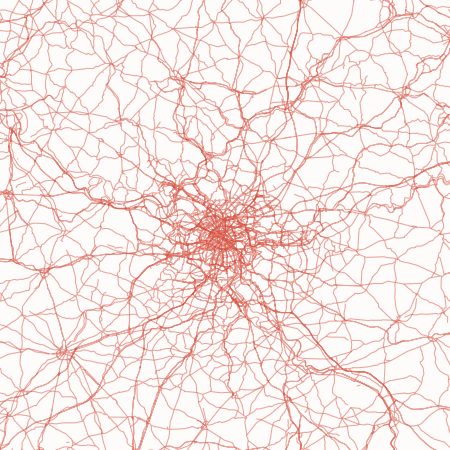
\includegraphics[width=1\textwidth]{images/schema/road_example}
      \caption{Road layer around Paris}
    \end{figure}
\end{minipage}

\begin{figure}[H]
  \centering
  \includegraphics[width=0.8\textwidth]{images/schema/road}
  \caption{Road layer schema}
\end{figure}



%------------------------------------------------------
\subsection{Buildings and Housenumbers}

\noindent\begin{minipage}[t]{0.48\linewidth}
    \vspace{0pt}
    Buildings are polygons such as houses or skyscrapers. They only appear on the highest zoom level 14 with the exception of large buildings already appearing at zoom level 13. Buildings are one of the most frequent features at high zoom levels.
    
    The \textbf{housenum\_label}  layer contains buildings or single points tagged with a housenumber. Housenumbers only appear on zoom level 14.

\end{minipage}
\hfill
\begin{minipage}[t]{0.48\linewidth}
    \vspace{-20pt}
    \begin{figure}[H]
      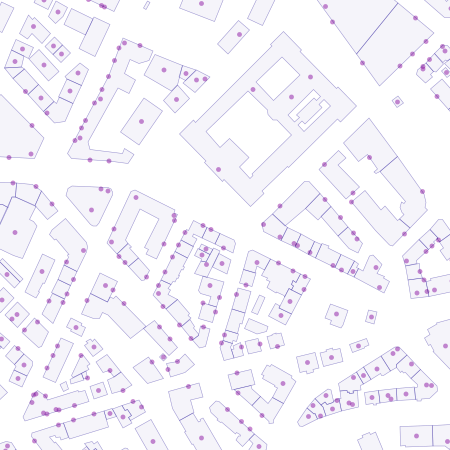
\includegraphics[width=1\textwidth]{images/schema/building_example}
      \caption{Buildings and house numbers}
    \end{figure}
\end{minipage}

\begin{figure}[H]
  \centering
  \includegraphics[width=0.8\textwidth]{images/schema/building}
  \caption{Building layer schema}
\end{figure}

%------------------------------------------------------
\subsection{Administrative Boundaries}

\noindent\begin{minipage}[t]{0.48\linewidth}
    \vspace{0pt}
    The \textbf{admin} layer contains the linestrings of administrative boundaries such as countries, states or provinces.
    Boundaries are treated as linestrings because borders often break in \osm{} and can no longer be reconstructed as polygons. Therefore it is safer to work with linestrings even though this provides less cartographic styling options.
    \\\\
    Since a different level of detail is required at different zoom levels the cultural data set from  Natural Earth \cite{16_naturalearthdata.com_2015} has been used at low zoom levels for boundaries of countries, provinces and disputed areas while at higher zoom levels the more accurate \osm{} data is used.
\end{minipage}
\hfill
\begin{minipage}[t]{0.48\linewidth}
    \vspace{-20pt}
    \begin{figure}[H]
      
\includegraphics[width=1\textwidth]{images/schema/admin_example}
      \caption{Admin level 4 (states) in the US}
    \end{figure}
\end{minipage}

\vspace{20}

\begin{figure}[H]
  \centering
  \includegraphics[width=1\textwidth]{images/schema/admin}
  \caption{Admin layer schema}
\end{figure}

%------------------------------------------------------
\subsection{Landuse and Landuse Overlay}

\noindent\begin{minipage}[t]{0.48\linewidth}
    \vspace{0pt}
    The layer \textbf{landuse} contains polygons of specially zoned land. The most frequent 
    features inside \textbf{landuse} are wood areas as well as national parks, swamps, commercial, industrial and military zones.
    Very large polygons are split into several pieces into the \textbf{landuse\_split\_polygon} table and large polygons are generalized
    for lower zoom levels. The polygons in the \textbf{landuse} layer are filtered by area depending on the zoom level so that at low zoom levels only the biggest polygons are shown.
\end{minipage}
\hfill
\begin{minipage}[t]{0.48\linewidth}
    \vspace{-20pt}
    \begin{figure}[H]
      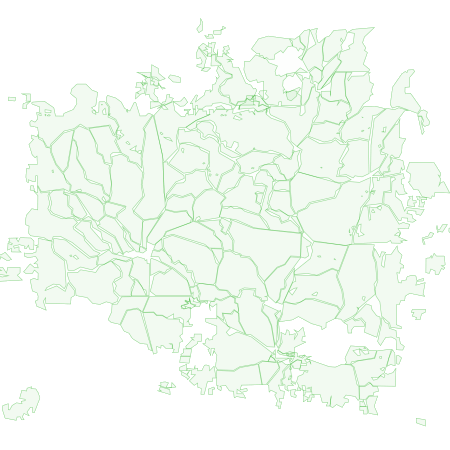
\includegraphics[width=1\textwidth]{images/schema/landuse_example}
      \caption{Landuse (wood) at zoom level 10}
    \end{figure}
\end{minipage}

\begin{figure}[H]
  \centering
  \includegraphics[width=0.8\textwidth]{images/schema/landuse}
  \caption{Landuse layer schema}
\end{figure}

%------------------------------------------------------
\subsection{POI Labels}

\noindent\begin{minipage}[t]{0.48\linewidth}
    \vspace{0pt}
    A point of interest (POI) is a feature bound to a particular point of the map (e.g. churches, schools, tourist attractions, hotels, trees).
    Not all POIs mapped in \osm{} are relevant for a visual map. In order to appear on the map, POIs are required to have at least a name or icon derived by the \textbf{type} field.
    \\\\
    Users shouldn't be overwhelmed with too many point of interest icons. Therefore the field \textbf{localrank} contains an ascending importance rank which can be used by map clients to prioritize important POIs. Very prominent POIs additionally have a scalerank based on their covered \textbf{area}. The rank calculation for POIs works very similar to place label ranking described in \autoref{place_label_rank_calc}.
\end{minipage}
\hfill
\begin{minipage}[t]{0.48\linewidth}
    \vspace{0pt}
    \begin{figure}[H]
        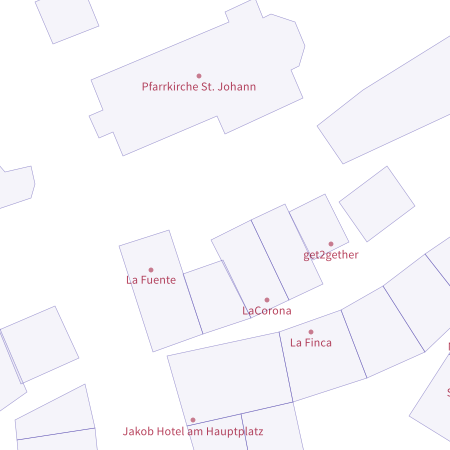
\includegraphics[width=\textwidth]{images/schema/poi_label_example}
        \caption{POI layer on top of building layer}
    \end{figure}
\end{minipage}
\vspace{20pt}
\begin{figure}[h]
  \centering
  \includegraphics[width=0.8\textwidth]{images/schema/poi_label}
  \caption{POI label layer schema}
\end{figure}

%---------------------------------
\subsection{Countries and States}

\noindent\begin{minipage}[t]{0.48\linewidth}
    \vspace{0pt}
    The placement and importance of labels of countries, states and seas matters\cite{12_axismaps.github.io_2015} and is important to get right. 
    Because it is difficult to ensure the quality of these features when importing directly from \osm{}, the labels of countries and states are curated by hand.\\
    Data from the Overpass API \cite{13_wiki.openstreetmap.org_2015} is converted into GeoJSON and manually edited and enhanced with a label rank to get the best possible label placement and importance ranking.
    This effort is worth it because country and state data changes
    at infrequent intervals.
    Country labels are not present on all zoom levels and are filtered based
    on their \textbf{scalerank} value to show countries like Italy prior to a less important city state like the Vatican.
\end{minipage}
\hfill
\begin{minipage}[t]{0.48\linewidth}
    \vspace{0pt}
    \begin{figure}[H]
        \includegraphics[width=\textwidth]{images/schema/country_state_label_example}
        \caption{Country and state labels around Brasil}
    \end{figure}
\end{minipage}

\begin{figure}[H]
  \centering
  \includegraphics[width=0.8\textwidth]{images/schema/country_state}
  \caption{Country and state layer schema}
\end{figure}

%------------------------------------------------------
\subsection{Places}

\noindent\begin{minipage}[t]{0.48\linewidth}
    \vspace{0pt}
    Place labels are vital for building nice maps with good text hierarchy.
    It is important to show only world cities at low zoom levels and then gradually show more and more local places. Filtering happens via the \textbf{scalerank} and \textbf{localrank} fields in the vector tiles. The \textbf{scalerank} field originates from the \textbf{ne\_10m\_populated\_places} table from NaturalEarth and is merged into the \textbf{place\_point} table. Most place labels are mapped as point in \osm{} except for residential districts and islands for which the centroid of the geometry is used as label point.
    Since place labels are very delicate and important
    every zoom level has custom filters to control which places are relevant.
    The rank calculation for places is explained in \autoref{place_label_rank_calc}.
\end{minipage}
\hfill
\begin{minipage}[t]{0.48\linewidth}
    \begin{figure}[H]
      \includegraphics[width=1\textwidth]{images/schema/place_example}
      \caption{Important place labels in Europe}
    \end{figure}
\end{minipage}

\begin{figure}[H]
  \centering
  \includegraphics[width=0.8\textwidth]{images/schema/place_label}
  \caption{Place label layer}
\end{figure}

%------------------------------------------------------
\subsection{Aeroways and Airports}

\noindent\begin{minipage}[t]{0.48\linewidth}
    \vspace{0pt}
    The layer \textbf{aeroway} contains infrastructure regarding air travel. The most common features are airports and their aprons, runways and taxiways. Airports are big landmarks and therefore all features are already present after zoom level 10. The layer consists of polygons and linestrings because runways are often polygons, while taxiways are mostly linestrings.\\
    The layer \textbf{airport\_label} contains labels of airports (either a point or the centroid of the airport polygon) since airports are important orientation points. The \textbf{scalerank} field describes the importance of the airport based on the covered area and type.
    Airports usually have official abbreviations (either the IATA, FAA, ICAO or custom reference code) that are stored in the \textbf{ref} field.
\end{minipage}
\hfill
\begin{minipage}[t]{0.48\linewidth}
    \vspace{-20pt}
    \begin{figure}[H]
      \centering
      \includegraphics[width=1\textwidth]{images/schema/aeroway_example}
      \caption{Aeroway and airport label layer of Zurich airport}
    \end{figure}
\end{minipage}

\begin{figure}[H]
  \centering
  \includegraphics[width=0.8\textwidth]{images/schema/aeroway}
  \caption{Aeroway layer}
\end{figure}

\begin{figure}[H]
  \centering
  \includegraphics[width=0.8\textwidth]{images/schema/airport}
  \caption{Airport label layer}
\end{figure}

%------------------------------------------------------
\subsection{Oceans, large Lakes and Bays}

\noindent\begin{minipage}[t]{0.48\linewidth}
    \vspace{0pt}
    For oceans, large lakes and bays having a curved label along the body is advantageous because the label does not interfere with other labels like places.
    \\
    Since these features are not available as polygons the label linestrings cannot be calculated but had to be drawn by hand. For the 100+ most important lakes and bays custom linestrings have been drawn. The metadata still originates from \osm{} but the geometries are custom. Since these natural features do not change this does not pose a problem. 
    \\
    The linestrings are filtered ascending for the upper zoom levels based on the \textbf{rank} field and are only shown at low zoom levels 0 to 6.
\end{minipage}
\hfill
\begin{minipage}[t]{0.48\linewidth}
    \vspace{-15pt}
    \begin{figure}[H]
      \includegraphics[width=1\textwidth]{images/schema/marine_label_example}
      \caption{Marine label of Mediterranean Sea}
    \end{figure}
\end{minipage}

\begin{figure}[H]
  \centering
  \includegraphics[width=0.8\textwidth]{images/schema/marine_label}
  \caption{Marine label layer}
\end{figure}

%------------------------------------------------------
\subsection{Mountain Peaks}

Mountain peaks are points tagged as mountains and volcanoes with a name and elevation. Because clients only have limited logic capabilities the elevation is calculated in both meters and feet.

\begin{figure}[H]
  \centering
  \includegraphics[width=0.8\textwidth]{images/schema/mountain_peak}
  \caption{Mountain peak label layer}
\end{figure}

%------------------------------------------------------
\subsection{Rail Stations}

Rail stations include railways, metros and tram stations. Since these
public transport features are usually styled differently than other point of
interests they are contained in a separate \textbf{rail\_station\_label\_layer}.

\begin{figure}[H]
  \centering
  \includegraphics[width=0.8\textwidth]{images/schema/rail_station}
  \caption{Rail station label layer}
\end{figure}\newpage
%\chapter{Results and Future}\label{part2_results_and_future}

\section{Results}\label{part2_results}
The result of this study thesis are described in Part 1, \hyperref[part1_results]{\emph{section 4.1}}.

\section{Future Development}\label{part2_future_development}

\subsection{Improvements}\label{small_improvements}
 
\subsection{New Features}\label{new_features}

\newpage{}\newpage
\chapter{Project Management}\label{project-management}

\section{Software Development Process}


An agile approach based on SCRUM has been used as the process model of this project.
The maintainers of the project act as joint product owners while the backlog is managed not only
by the product owners but also by the community which add features to the wish list and even contribute code to the repository.\\
At the beginning of each sprint features of the backlog are estimated and scheduled for the next release. After each sprint (two to three weeks) a new stable version is released.\\
In comparison to SCRUM there are no sprint reviews and retroperspective but regular meetings with the thesis advisor to inform about project status are conducted.
Regular meetings with the technical advisor help to solve problems together.

\subsection*{GitHub}\label{github}
GitHub was used for planning and tracking of the tasks and milestones.
To provide a SCRUM board and burndown chart the ZenHub browser plugin has been used.


It has a big advantage over other project management tools, as revision control and issue tracking are at the same place.
Non project members can understand the thoughts behind certain decisions and communicate their ideas directly to team members which is important for an open source project.\\

An organization named osm2vectortiles has been created with the following repositories:

\begin{itemize}
\item
  \textbf{osm2vectortiles} Contains the dsitributed workflow to create vector tiles
\item
  \textbf{tileserver-gl-light} A trimmed down fork of tileserver-gl for serving MBTiles and predefined Mapbox GL styles with emphasis on serving vector tiles from \osmvt{}
\item
  \textbf{imposm3} Custom fork of imposm3 to support timestamp field
\item
  \textbf{mapbox-gl-styles} Collection of Mapbox GL styles that are compatible with \osmvt{}.
\item
  \textbf{rabbitmq} Custom fork of official RabbitMQ Docker image with additional support for message timeout configuration
\item
  \textbf{bachelor-thesis} LaTeX source for bachelor thesis
\item
  \textbf{study-thesis} LaTeX source for preceding study thesis
\end{itemize}

\section{Schedule}

Because the \osmvt{} members where already familiar with the technologies and field of work no elaboration phase was needed. Each sprint was tightly coupled to the next release.

\section{Milestones}

Each milestones marks a special release version of the vector tiles.

\begin{table}[H]
\centering
    \begin{tabular}{p{1.5cm} p{1.5cm} p{1.5cm} p{1.5cm} p{1.5cm}}
    Version & Date  & Resolved Issues & Merged PRs & Fixed Bugs\\
    \hline
    v1.1   & Mar 4  & 9 & 3 & 1 \\
    v1.2   & Mar 21 & 9 & 5 & 1 \\
    v1.3   & Apr 1  & 6 & 6 & 1 \\
    v1.4   & Apr 12 & 14 & 11 & 6 \\
    v1.4.1 & Apr 22 & 10 & 11 & 10 \\
    v1.4.2 & Apr 25 & 5 & 4 & 11 \\
    v1.5   & Apr 28 & 5 & 8 & 3 \\
    v2.0   & May 24 & 12 & 8 & 4 \\
    \end{tabular}
    \caption[Milestones]{Project sprints and statistics}
\end{table}

\section{Roles and Responsibilities}\label{roles-and-responsibilities}

\begin{table}[H]
\centering
    \begin{tabular}{p{3cm} p{9.5cm}}
Prof Stefan Keller & Thesis advisor responsible for supervising work and
assess the thesis.\\ \hline
Petr Pridal, PhD &
Technical partner responsible for providing infrastructure \\ \hline
Manuel Roth &
Maintainer\\ \hline
Lukas Martinelli &
Maintainer\\ \hline
    \end{tabular}
    \caption{Thesis contributors and their roles}
\end{table}

\section{Risks}\label{risks}

In contrast to the preceding study thesis the bachelor thesis is less risky due
to the increased knowledge of the field.

\begin{table}[H]
\centering
    \begin{tabular}{p{4.5cm} p{7.5cm} p{1.8cm}}
    \hline
    Risk & Measurement & Probability (1-6)\\
    \hline
    Too slow update process& Early measurements of solution & 4\\
    Vector tiles oversized & Continuously measure vector tiles & 4\\
    Infrastructure not sufficient & Switch to non school infrastructure and rely on external sponsors & 3\\
    Unwanted Features & Open roadmap and feedback of community & 2\\
    Lacking quality & Regularly control whether defined quality measurements were complied with & 2\\
    \end{tabular}
    \caption{Risks and measurements}
\end{table}
\newpage
\chapter{Quality Measures}\label{quality-measures}

Visual Test
Strutural Test
Report Tool
Coding Standards

\section{Testing}\label{testing}

The osm2vectortiles ecosystem is quite diverse with a big collection of small tools that all work together which makes testing really complex.

\subsection{Integration Test}

In Travis CI\cite{pm_5_travis-ci.org_2015}  the entire workflow was completed for a small data sample on each commit.
Because the entire workflow is configured with Docker Compose \cite{pm_6_docs.docker.com_2015} the CI server had to execute all import steps in serial order. This is a straightforward way to check if all components work together correctly
and although it is a simple setup it has helped tremendously during project development, catching bugs
like missing tables or SQL typos.

\begin{yamlcode}
script:
  # Test import
  - docker-compose up -d postgis
  - sleep 10
  - docker-compose run import-external
  - docker-compose run import-osm
  - docker-compose run import-sql
  # Test export
  - docker-compose run export
  # Test changed tiles
  - docker-compose run update-osm-diff
  - docker-compose run import-osm-diff
  - docker-compose run changed-tiles
\end{yamlcode}

\subsection{Visual Testing}

\begin{figure}[H]
  \centering
  \includegraphics[width=1.0\textwidth]{images/visual_compare}
  \caption{Visual Compare Tool}
  \label{visual_compare} 
\end{figure}

\section{Guidelines}\label{guidelines}
To have homogeneous software the contributors have settled on common guidelines in the beginning of the project.

\subsection{Releases}
Semantic versioning \cite{pm_7_preston-werner_2015} should be used for releases.
At the end of each milestone a new release will be created.
\newpage

\subsection{Git}\label{git}
\paragraph{Commit Messages}
The seven rules of great git commit
messages\cite{pm_8_chris.beams.io_2015} should be used.

\paragraph{Rewriting}
Git history should be kept clean and therefore local branches should be
squashed meaningfully.

\paragraph{Pulling}
To avoid unnecessary merge messages one should always use the
\texttt{-\/-rebase} parameter.

\subsection{Workflow}\label{git-workflow}
The Feature Branch Workflow\cite{pm_9_atlassian_git_tutorial_2015} should be used. Every project member has a local repository with a copy of the remote
repository. For each feature ticket in GitHub a separate branch
will be created. Once a ticket has been completed a pull request will be
created and needs to be merged into the \texttt{master} branch by an other 

\subsection{Coding Standards}

\paragraph{Bash} Bash was used for the Docker image entrypoints and follow
the rules of Defensive Bash Programming \cite{pm_10_lavi_2012}.

\paragraph{Python} Python code should stay PEP-8\cite{pm_11_python.org_2015} compliant and write idiomatic Python code according to PEP-20\cite{pm_12_python.org_2015}.

\paragraph{JavaScript} The JavaScript code is checked using ESLint\cite{pm_13_eslint.org_2015}

\paragraph{SQL} The PostgreSQL code is using upper case for the key words. Apart from nice formatted SQL code and functions should be used
to keep the queries DRY\cite{pm_14_wikipedia_2015}.

\paragraph{Dockerfile} Dockerfiles follow the best practices\cite{pm_15_docs.docker.com_2015} defined by Docker.
\newpage
\chapter{Project Monitoring}\label{project monitoring}

\section{Code Statistics}



\section{Estimated Time vs Actual Time}

Our estimations were too optimistic. Due to the extensive
training period required to get started in a GIS environment
the actual time was more than originally estimated.


\begin{table}[H]
\centering
    \begin{tabular}{lll}
    \textbf{Sprint}        & \textbf{Estimated} & \textbf{Actual} \\
     \hline
    v1.1  & 80     & 16        \\
    v1.2  & 80     & 55        \\
    v1.3  & 80     & 50        \\
    v1.4  & 80     & 102       \\
    v1.5  & 80     & 106         \\
    v1.6  & 80     & 53        \\
    \hline
    \textbf{Total} & 720 & 720 \\
    \end{tabular}
    \caption{Estimated vs actual time for different sprints}
\end{table}
\newpage

\section{Time per Person}

Both contributors invested about the same amount of time.

\begin{table}[H]
\centering
    \begin{tabular}{llll}
    \textbf{Sprint}  & \textbf{Lukas Martinelli} & \textbf{Manuel Roth} & \textbf{Total} \\
    \hline
    v1.1    & 11               & 9           & 20    \\
    v1.2    & 22               & 21          & 43    \\
    v1.3    & 25               & 23          & 48    \\
    v1.4    & 56               & 65          & 121   \\
    v1.5    & 77               & 75          & 152   \\
    v1.6    & 27               & 21          & 48    \\
    \hline
    \textbf{Total}          & 245              & 248         & 493   \\
    \end{tabular}
    \caption{Time for each contributor for sprints}
\end{table}\newpage
\chapter{Developer and User Documentation}

During the study thesis detailed documentation and tutorials for the \osmvt{} project has been created. The documentation was separated into a user-centric and developer-centric part.
All of this information was provided on the project website (\url{http://osm2vectortiles.org}). However when the project was publicly released and people started to get interested in the project, two main problems occurred:

\begin{itemize}
    \item The tutorials targeted at regular users were too complicated and error prone
    \item Developers want to have the documentation on GitHub right next to the code and not on the project website
\end{itemize}

With this knowledge it was decided to move the developer-centric documentation into README files right next to the code and simplify the user-centric tutorials to eliminate most beginner errors.

\begin{figure}[H]
  \centering
  \includegraphics[width=1.0\textwidth]{images/documentation/developer_documentation}
  \caption{Documentation of the export component using a README file}
  \label{developer_documentation}
\end{figure}

\autoref{developer_documentation} and \autoref{user_documentation} show the documentation in the repository on GitHub and on the project website. The documentation can be found either on GitHub (\url{https://github.com/osm2vectortiles/osm2vectortiles}) or on the project website (\url{http://osm2vectortiles.org}).

\begin{figure}[H]
  \centering
  \includegraphics[width=1.0\textwidth]{images/documentation/user_documentation}
  \caption{Simplified overview of user documentation on the project website}
  \label{user_documentation}
\end{figure}\newpage

%------------------------------------------------
%	THESIS CONTENT - APPENDICES
%------------------------------------------------
\newpage
\appendix
\part{Appendix}
\includepdf[pages={1}]{images/project_proposal.pdf}
%\chapter*{Meeting Protocols}

\section*{7th September 2015}

\subsection*{Participants}
\begin{itemize}
  \item Petr Pridal
  \item Stefan Keller
  \item Lukas Martinelli
  \item Manuel Roth
\end{itemize}


\subsection*{Talking points}

\begin{itemize}
  \item Get to know each other
  \item Project goal
  \item Architecture of Docker containers
  \item Definition of tasks and milestones
\end{itemize}

\section*{16th September 2015}

\subsection*{Participants}

\begin{itemize}
  \item Stefan Keller
  \item Lukas Martinelli
  \item Manuel Roth
\end{itemize}


\subsection*{Talking points}

\begin{itemize}
  \item Language choice of thesis
  \item Similarity of documentation to SE2 project
  \item Role of Petr Pidal
  \item Mechanics of MBTiles
\end{itemize}

\subsection*{Protocol}
\begin{itemize}
  \item Create a project proposal
  \item Inform ourselves about Meta Tiles
  \item Few prerendered tiles can cover most of the used map
  \item Before each meeting, send email with done, difficulties and plan for next week to Stefan Keller
  \item Thesis of prior years can be found at HSR eprints
\end{itemize}


\subsection*{Questions and Answers}

- Can the thesis be written in English?
\textit{Yes, that's up to you. Other groups did write their project documentation in English and the actual thesis in German.}

- Should the documentation be made similar to SE2?
\textit{Yes, but only the parts with make sense to your project. Usually, the thesis is divided into two parts, the first part should be like an article of a computer magazine (C't). The second part all formal documents (requirements analysis, domain analysis, use cases)}

- What's Mr.Pridal's role? - Does Mr.Pridal affect the evaluation?
\textit{Mr.Pridal can basically be viewed as an industrial partner. I will seek his opinion at the end of the project. If there should be differences between you and him, I will have the final word.}

\section*{25th September 2015}

\subsection*{Participants}

\begin{itemize}
  \item Stefan Keller
  \item Lukas Martinelli
  \item Manuel Roth
\end{itemize}


\subsection*{Done}

\begin{itemize}
  \item Went through OSM Workflow ( OSM Source -> Import OSM Data -> Postgis -> Source Project -> Export mbtiles -> Serving mbtiles)
\end{itemize}

\subsection*{Difficulties}

\begin{itemize}
  \item It was not clear, if we could take an existing source project or if we had to make our own.
\end{itemize}

\subsection*{Plan}

\begin{itemize}
  \item Documenting OSM Workflow
  \item Comparing osm2pgsql and imposm3
  \item Meeting with Petr Pridal on Monday
\end{itemize}

\subsection*{Talking points}

\begin{itemize}
  \item Imposm3 or osm2pgsql vor import: many people in the OSM community are used to osm2pgsql and its default schema (point, line, polygon, road). The criteria for choosing the import tool, should be efficient and have the possibility to update data with OSM diff files.
  \item Thesis should compare GeoPackage and MBTiles 
  \item Term feature set is more accurate than layer
\end{itemize}

\section*{28th September 2015}

\subsection*{Participants}

\begin{itemize}
  \item Petr Pridal
  \item Lukas Martinelli
  \item Manuel Roth
\end{itemize}


\subsection*{Done}

\begin{itemize}
  \item Reached alpha milestone(first version of components)
\end{itemize}

\subsection*{Difficulties}

\begin{itemize}
  \item We need to define system requirements for the containers
  \item On small machines(> 500 RAM) null pointer exceptions while importing with imposm3
  \item What is the purpose of the debug viewer
\end{itemize}

\subsection*{Plan}

\begin{itemize}
  \item Next meeting with Petr: Monday 5pm, 19th of October 2015
  \item Decision of which rendering and tile serving stack should be choosen (based on performance tests with each stack)
\end{itemize}

\subsection*{Talking points}

\begin{itemize}
  \item Can current software stack meet our requirements?
  \subitem Requirements osm2vectortile stack: Render whoule planet in reasonable amount of time(less than one month)
  \subitem Requirements tileserver: not yet defined
  \item Performance:
  \subitem Compare Vector tile rendering stack with wikimedia's
  \subsubitem Import only necessary data for rendering
  \subsubitem Compare your source project with wikimedia's
  \subsubitem Why did wikimedia fork mapbox's osm-brigt style?
  \subitem Tileserver: Compare performance of node + nginx with apache + renderd
  \item The debug viewer is needed, if you want to view the mbtiles without Mapbox studio
  \subitem Petr would be interested to integrate thiw viewer into tileserver-php
  \item Rename tileserver to vtileserver for clarity
\end{itemize}

\section*{2th October 2015}

\subsection*{Participants}

\begin{itemize}
  \item Stefan Keller
  \item Manuel Roth
\end{itemize}


\subsection*{Done}

\begin{itemize}
  \item Documented OSM worklow
  \item Meeting with Petr
  \item OSM Planet file imported
  \item Passed alpha milestone
\end{itemize}

\subsection*{Difficulties}

\begin{itemize}
  \item OSX postgres volume mounting problem
\end{itemize}

\subsection*{Plan}

\begin{itemize}
  \item Compare Wikimedia OSM stack with current stack (performance)
  \item Decision of which rendering and tile serving stack should be choosen (based on performance tests with each stack)
\end{itemize}

\subsection*{Questions and Answers}

- How many hours does each of us has to invest into the thesis?
\textit{Every team member has to invest at least 240h into the thesis (8 ECTS * 30h)}

- On which server can we generate the mbtiles and how up-to-date should they be? (weekly updates)
\textit{You can use the IFS server for the mbtiles generation. If there are problems with the server, please contact Mirko Stocker. There are no special requirements for how current the mbtiles have to be}

\subsection*{Talking points}
\begin{itemize}
  \item Stefan Keller creates the project proposal and sends it for review back to us. On next weeks meeting we are going to sign the project proposal.
  \item Stefan Keller's contact person at wikimedia maps: Tim alias Kolossos (tim@alder-digital.de)
\end{itemize}

\section*{16th October 2015}

\subsection*{Participants}

\begin{itemize}
  \item Stefan Keller
  \item Lukas Martinelli
  \item Manuel Roth
\end{itemize}


\subsection*{Done}

\begin{itemize}
  \item Structure of thesis defined
  \item Debug Viewer created
  \item Import performance analysis
  \item Performance scenarios for vector tile server defined (Gatling.io)
\end{itemize}

\subsection*{Difficulties}

\begin{itemize}
  \item Mapnik with vector tiles as source
  \item SQL queries are bottleneck of mbtiles creation
\end{itemize}

\subsection*{Plan}

\begin{itemize}
  \item Performance tests with tessera and apache tile server
  \item Mbtiles for whole switzerland
\end{itemize}

\section*{30th October 2015}

\subsection*{Participants}

\begin{itemize}
  \item Stefan Keller
  \item Lukas Martinelli
  \item Manuel Roth
\end{itemize}

\subsection*{Done}

\begin{itemize}
  \item Started with data style
  \item Created tool to analyze mapbox streets vector tiles
  \item Started working on zoom level 14
  \item Added lots of data to data style
\end{itemize}

\subsection*{Difficulties}

\begin{itemize}
  \item Find differences to our vector tiles
\end{itemize}

\subsection*{Plan}

\begin{itemize}
  \item Identify missing items/layers
  \item Update data style
\end{itemize}


\section*{13th November 2015}

\subsection*{Participants}

\begin{itemize}
  \item Stefan Keller
  \item Lukas Martinelli
  \item Manuel Roth
\end{itemize}

\subsection*{Done}

\begin{itemize}
  \item Work on zoom level 14 is almost finished
  \item Work on zoom level 10 to 13 has started
  \item Chapter technical report started
\end{itemize}

\subsection*{Plan}

\begin{itemize}
  \item Finish zoom level 10 to 13
  \item Work from lowest zoom level(14) to smallest zoom level(0)
  \item Finish chapter technical report
\end{itemize}

\section*{27th November 2015}

\subsection*{Participants}

\begin{itemize}
  \item Stefan Keller
  \item Lukas Martinelli
  \item Manuel Roth
\end{itemize}

\subsection*{Done}

\begin{itemize}
  \item Work on zoom level 10 to 13 is finished
  \item Work on zoom level 0 to 10 has started with additional data source
  \item Chapter project documentation started
\end{itemize}

\subsection*{Difficulties}

\begin{itemize}
  \item For upper zoom levels Natural Earth data set is needed (0-8)
\end{itemize}

\subsection*{Plan}

\begin{itemize}
  \item Finish zoom level 0 to 10
  \item Finish chapter project documentation
\end{itemize}

\section*{11th December 2015}

\subsection*{Participants}

\begin{itemize}
  \item Stefan Keller
  \item Lukas Martinelli
  \item Manuel Roth
\end{itemize}

\subsection*{Done}

\begin{itemize}
  \item Finished work on data style
  \item Chapter technical report, project documentation finished
  \item Draft of chapter project management created
\end{itemize}

\subsection*{Plan}

\begin{itemize}
  \item Finish chapter project management
  \item Revise thesis with feedback 
  \item Create extracts for project website
  \item Create user guide
\end{itemize}

\section*{18th December 2015}

\subsection*{Participants}

\begin{itemize}
  \item Stefan Keller
  \item Lukas Martinelli
  \item Manuel Roth
\end{itemize}

\subsection*{Done}

\begin{itemize}
  \item Fished project thesis
  \item Launched project website
  \item Launched project with press release (social media, blogs)
  \item Created cd, poster, added thesis to HSR abstract tool
\end{itemize}

\newpage{}\newpage

%---------------------------------------
%	POST-CONTENT THESIS PAGES
%---------------------------------------
% Bibliography

\label{app:bibliography} % Reference the bibliography elsewhere with \autoref{app:bibliography}
\raggedright
\manualmark
\markboth{\spacedlowsmallcaps{\bibname}}{\spacedlowsmallcaps{\bibname}} 
\refstepcounter{dummy}

\addtocontents{toc}{\protect\vspace{\beforebibskip}} % Place the bibliography slightly below the rest of the document content in the table of contents
\addcontentsline{toc}{chapter}{\tocEntry{\bibname}}

\bibliographystyle{plainnat}
\bibliography{bibliography}

\newpage
% Declaration

\refstepcounter{dummy}
\pdfbookmark[0]{Declaration}{declaration} % Bookmark name visible in a PDF viewer

\chapter*{Declaration} % Declaration section text

\thispagestyle{empty}

Hereby we acknowledge,

\begin{itemize}
		\item that we conducted this thesis by ourselves and without any external help,
			except with those, which are explicitly mentioned,
		\item that all used sources are cited academically correct, and 
		\item that I didn't use any copyright protected materials (e.g. images) in
			an unauthorized manner.
\end{itemize}

\bigskip
 
\noindent\textit{\myLocation, \myTime}

\bigskip

\begin{flushright}
    \begin{tabular}{m{8cm}}
    \hspace{1cm}\includegraphics[width=.5\textwidth]{images/signature_lukas.jpg}
    \\ \hline
    \centering Lukas Martinelli, \today \\
    \end{tabular}
\end{flushright}

\begin{flushright}
    \begin{tabular}{m{8cm}}
    \hspace{2cm}\includegraphics[width=.33\textwidth]{images/signature_manuel.png}
    \\ \hline
    \centering Manuel Roth, \today \\
    \end{tabular}
\end{flushright}



%---------------------------------------

\end{document}